% MIT License

% Copyright (c) 2019-2020 Simon Crase

% Permission is hereby granted, free of charge, to any person obtaining a copy
% of this software and associated documentation files (the "Software"), to deal
% in the Software without restriction, including without limitation the rights
% to use, copy, modify, merge, publish, distribute, sublicense, and/or sell
% copies of the Software, and to permit persons to whom the Software is
% furnished to do so, subject to the following conditions:

% The above copyright notice and this permission notice shall be included in all
% copies or substantial portions of the Software.

% THE SOFTWARE IS PROVIDED "AS IS", WITHOUT WARRANTY OF ANY KIND, EXPRESS OR
% IMPLIED, INCLUDING BUT NOT LIMITED TO THE WARRANTIES OF MERCHANTABILITY,
% FITNESS FOR A PARTICULAR PURPOSE AND NONINFRINGEMENT. IN NO EVENT SHALL THE
% AUTHORS OR COPYRIGHT HOLDERS BE LIABLE FOR ANY CLAIM, DAMAGES OR OTHER
% LIABILITY, WHETHER IN AN ACTION OF CONTRACT, TORT OR OTHERWISE, ARISING FROM,
% OUT OF OR IN CONNECTION WITH THE SOFTWARE OR THE USE OR OTHER DEALINGS IN THE
% SOFTWARE.

\documentclass[]{article}
\usepackage{caption,subcaption,graphicx,float,url,amsmath,amssymb,tocloft}
\usepackage[hidelinks]{hyperref}
\usepackage[toc,acronym,nonumberlist]{glossaries}
\usepackage{titling}
\setacronymstyle{long-short}
\usepackage{glossaries-extra}
\graphicspath{{figs/}} 
\setlength{\cftsubsecindent}{0em}
\setlength{\cftsecnumwidth}{3em}
\setlength{\cftsubsecnumwidth}{3em}
% I snarfed the next line from Stack exchange
% https://tex.stackexchange.com/questions
%    /42726/align-but-show-one-equation-number-at-the-end
% It allows me to suppress equation numbers with align*,
% then selectively add equation numbers
% for lines that I want to reference slsewhere
\newcommand\numberthis{\addtocounter{equation}{1}\tag{\theequation}}
% Add logo at start of document
\pretitle{
	\begin{center}
		
\includegraphics[width=6cm]{KanjiLife}\\	
	}
	\posttitle{\end{center}}

%opening
\title{
	Notes from Origins of Life\\
	Week 6\\
	 Astrobiology \& General Theories of Life
}
\author{Simon Crase (compiler)\\simon@greenweaves.nz}

\makeglossaries
% Prefix section numbers with week number
\renewcommand{\thesection}{6.\arabic{section}}

\loadglsentries{glossary-entries}

\renewcommand{\glstextformat}[1]{\textbf{\em #1}}

\begin{document}

\maketitle

\begin{abstract}
   These are my notes from the $6^{th}$ Week of the Santa Fe Institute Origins of Life Course\cite{sfi2020}. 
   The content and images contained herein are the intellectual property of the Santa Fe Institute, with the exception of any errors in transcription, which are my own.
   These notes are distributed in the hope that they will be useful,
   but without any warranty, and without even the implied warranty of
   merchantability or fitness for a particular purpose. All feedback is welcome,
   but I don't necessarily undertake to do anything with it.\\
   \LaTeX source for this week's lectures can be found at\\
   \url{https://github.com/weka511/complexity/tree/master/origins}.
\end{abstract}

\setcounter{tocdepth}{2}
\tableofcontents

\listoffigures

\section[Introduction]{Introduction--Chris Kempes}

Over the course of these lectures we have provided a range of tools and perspectives that would help us understand the origin of life on our own planet. These can be used to develop a general theory of life. Our ultimate goal is to provide a general theory of Life, one capable of uncovering the history we know about, but also bounding the possibilities for other types of life, and helping us recognize other forms of life. In this unit we'll discuss the search for life beyond Earth and how origins of life fits into this effort. We'll also discuss general evolutionary processes and abstract life. 

\section[Origins of Life and Astrobiology]{Origins of Life and Astrobiology-- Sara Imari Walker}

Hi I'm Sarah Walker, a professor at Arizona State University and an astrobiologist.
I study the origin of life. One of the questions you might have as an astrobiologist is: why is origin of life so critical to the study of astrobiology?

Astrobiologists are really interested in whether or not we can identify a living world, so if we can identify life on another planet.
We want to discover aliens and ultimately, the question is whether we'll be able to distinguish planets that have life from plants that don't have life. So in our own solar system, we can actually send robotic missions to other planets to look for life on the surface of those worlds but we're thinking about exoplanets and planets and distant solar systems all that we're going to get is a little bit of data about the entire planet.

As astrobiologists we are interested in thinking about life not only at the scale of individual organisms, but also at the scale of entire planets. 
And so just to talk about the magnitude of the problem a lot of people want to talk about looking at life in kind of new ways and maybe trying to use insights from different aspects of known fields of science to try to understand how we identify life.
Figure \ref{fig:Jupiter:Tellus} shows two worlds that are probably familiar to everyone, Jupiter and Earth; we know one of these planets is inhabited and the other isn't.
\begin{figure}[H]
	\caption[What makes worlds with life different?]{What makes worlds with life different? Not just non-equilibrium structures.}\label{fig:Jupiter:Tellus}
	\begin{subfigure}[b]{0.44\textwidth}
		\caption{Jupiter has its Great Red Spot}\label{fig:Jupiter}
		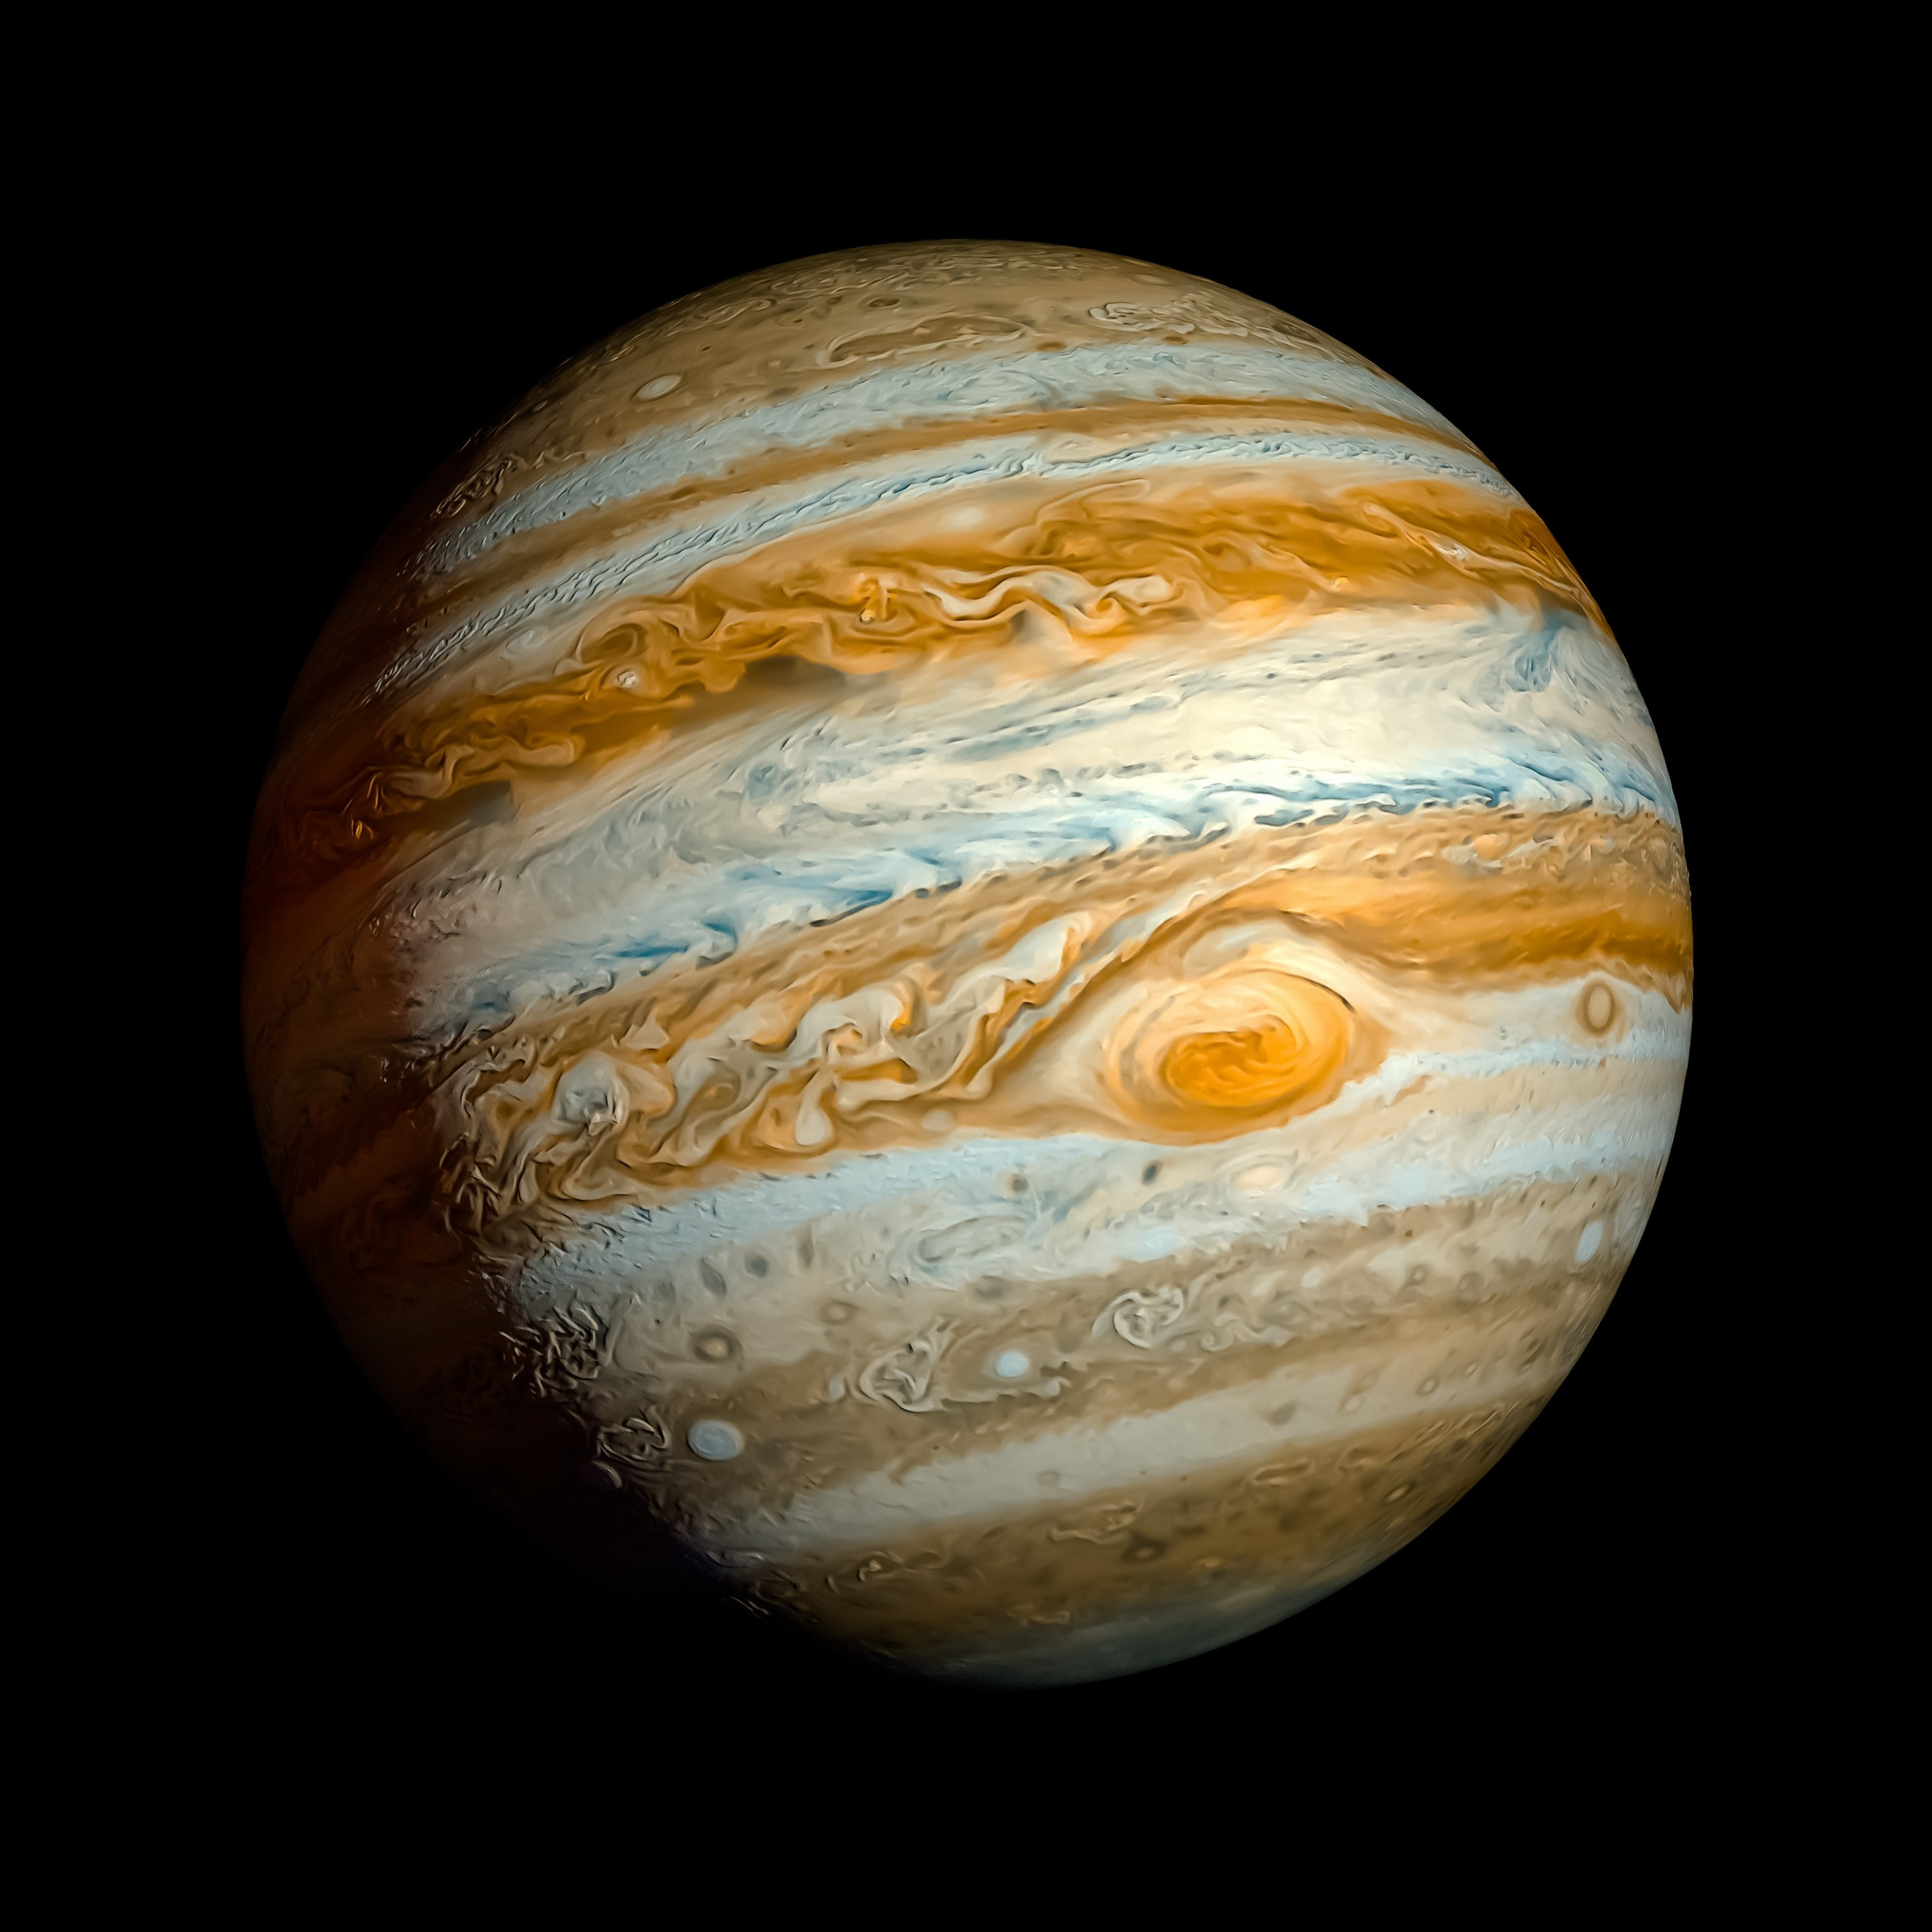
\includegraphics[width=\textwidth]{Jupiter}
	\end{subfigure}
	\;\;\;
	\begin{subfigure}[b]{0.5\textwidth}
		\caption{Earth at night, showing cities.}\label{fig:Earth}
		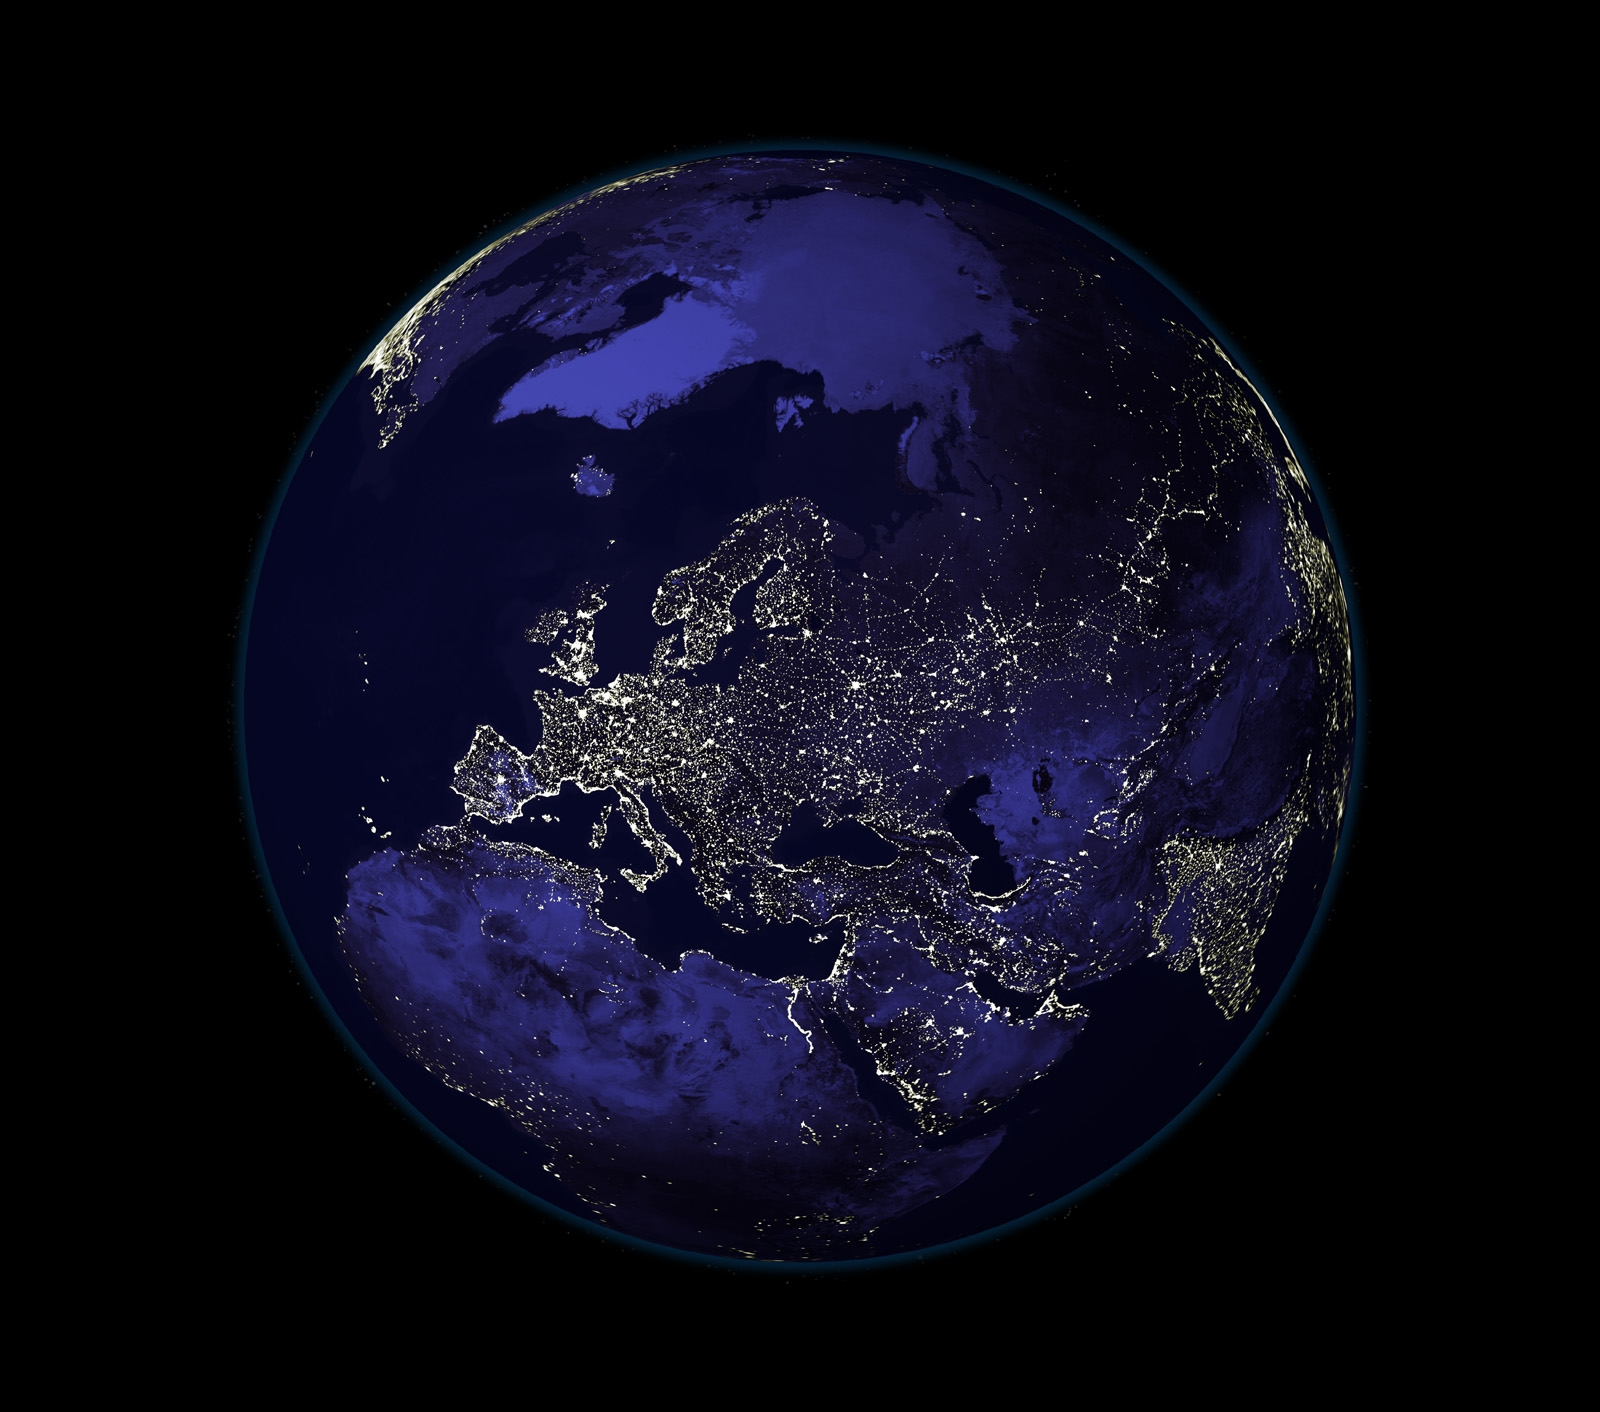
\includegraphics[width=\textwidth]{Tellus}
	\end{subfigure}
\end{figure}

The inhabited world is obviously our very own earth, and we can see living structures on its surface. What we see in Figure \ref{fig:Earth} is cities at night. When we're
thinking about how to think about the problem of distinguishing the living process on Earth from the nonliving process on Jupiter, it's clear that both have non-equilibrium structures on their surfaces. Jupiter--Figure \ref{fig:Jupiter} has this great red spot and Earth has cities. So when we want to talk about defining the properties of those planets that are associated with life, it's not just about this disequilibra. Clearly cities are fundamentally different from the great red spot of Jupiter, even though they're both non-equilibrium structures. So we have to move a little bit further and understand the origins of the processes that led to structure on the surface of our planet that are associated with life, and the root of that question is really to understand the probability of life emerging on a planet--Figure \ref{fig:P:Life}, and how can we actually understand that as a planetary scale process. 

\begin{figure}[H]
	\caption[Rate of abiogenesis in a prebiotic environment]{Rate of abiogenesis in a prebiotic environment as a function of its physical and chemical conditions}\label{fig:P:Life}
	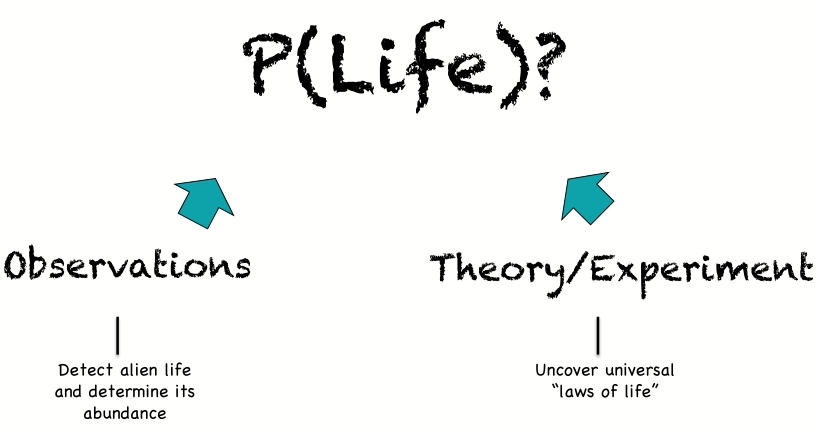
\includegraphics[width=0.9\textwidth]{P_Life}
\end{figure}


There's really two ways of constraining the likelihood of life emerging on a planet. We don't think that Jupiter is a living planet:
based on our observations of Jupiter, it \emph{might} turn out to satisfy some definition of life down the road if we actually come up with a theory for life and Jupiter satisfies that theory; right now we don't think Jupiter's alive.

And so we need some observations of other living world to constrain the probability of life. Right now Earth is the only example we know and so to do that we actually have to detect alien life and determine its abundance. And so this is the way you usually people think about astrobiology is actually looking at other worlds trying to identify if there's aliens on those worlds and then maybe we would actually be able to constrain the probability that a planet like Earth is going to emerge life on its surface and a planet like Jupiter is not. 

But we can also think about theory and experiment to constrain the probability for life. From this view the idea is really to try to uncover the universal principles of life that might actually allow us to build predictive models for the circumstances under which life should emerge. So, we would have some a priori theory that would enable us to predict $P(life)$--the probability of life emerging.
That theory should be able to account for the differences in Figure \ref{fig:Jupiter:Tellus}, i.e. to explain why it's not just a non-equilibrium process on the surface of a planet. In the case of formation of cities or forests--or any of the kind of rich structure that we see on earth that's a product of biology--the theory would be able to explain what those things are and be able to predict what kinds of other
examples of life we might be able to see on other planets and their likelihood.

But really what we're talking about in
order to constrain the probability of
life is not just to think about the
probability of forests or cities on the
surface of planets as opposed to the
probability of great red spots or other
kinds of dissipative structures that
aren't alive. What we really want is to
understand what's the likelihood of life
even emerging on that planet.
So we really need to be able to solve
the origin of life problem in order to do
astrobiology effectively and constrain
the likelihood of life in the universe.

And so in order to do that, we have to
come up with better theories for origins
of life and be able to understand how
life emerges. And so one of the ways I
like to think about it is really that
we're looking for new principles that
would explain life not just on earth but
life on other planets and I really love
this quote from David Deutsch which I
think articulates very nicely the kind
of processes that are happening on
planets that we really need to be able
to understand in order to understand
life. 

\begin{quotation}
	Base metals can be transmuted into gold by stars, and by intelligent beings who understand the processes that power stars, and by nothing else in the universe--David Deutsch\cite{deutsch2011beginning}.
\end{quotation}

We have a physics that explains things like stars or the physics of Jupiter and why Jupiter has a great storm on the surface of the planet at the great red spot.
But we don't have a physics that explains the evolution of a planet like our own, how life emerges on that planet, or how it evolves over time to lead to the kind of diversity of structures that we have on the surface of our planet today, like cities and
thinking human beings.

\begin{figure}[H]
	\begin{center}
		\caption[We don't have a physics that explains the evolution of our planet]{We don't have a physics that explains the evolution of a planet like our own}\label{fig:tellus}
		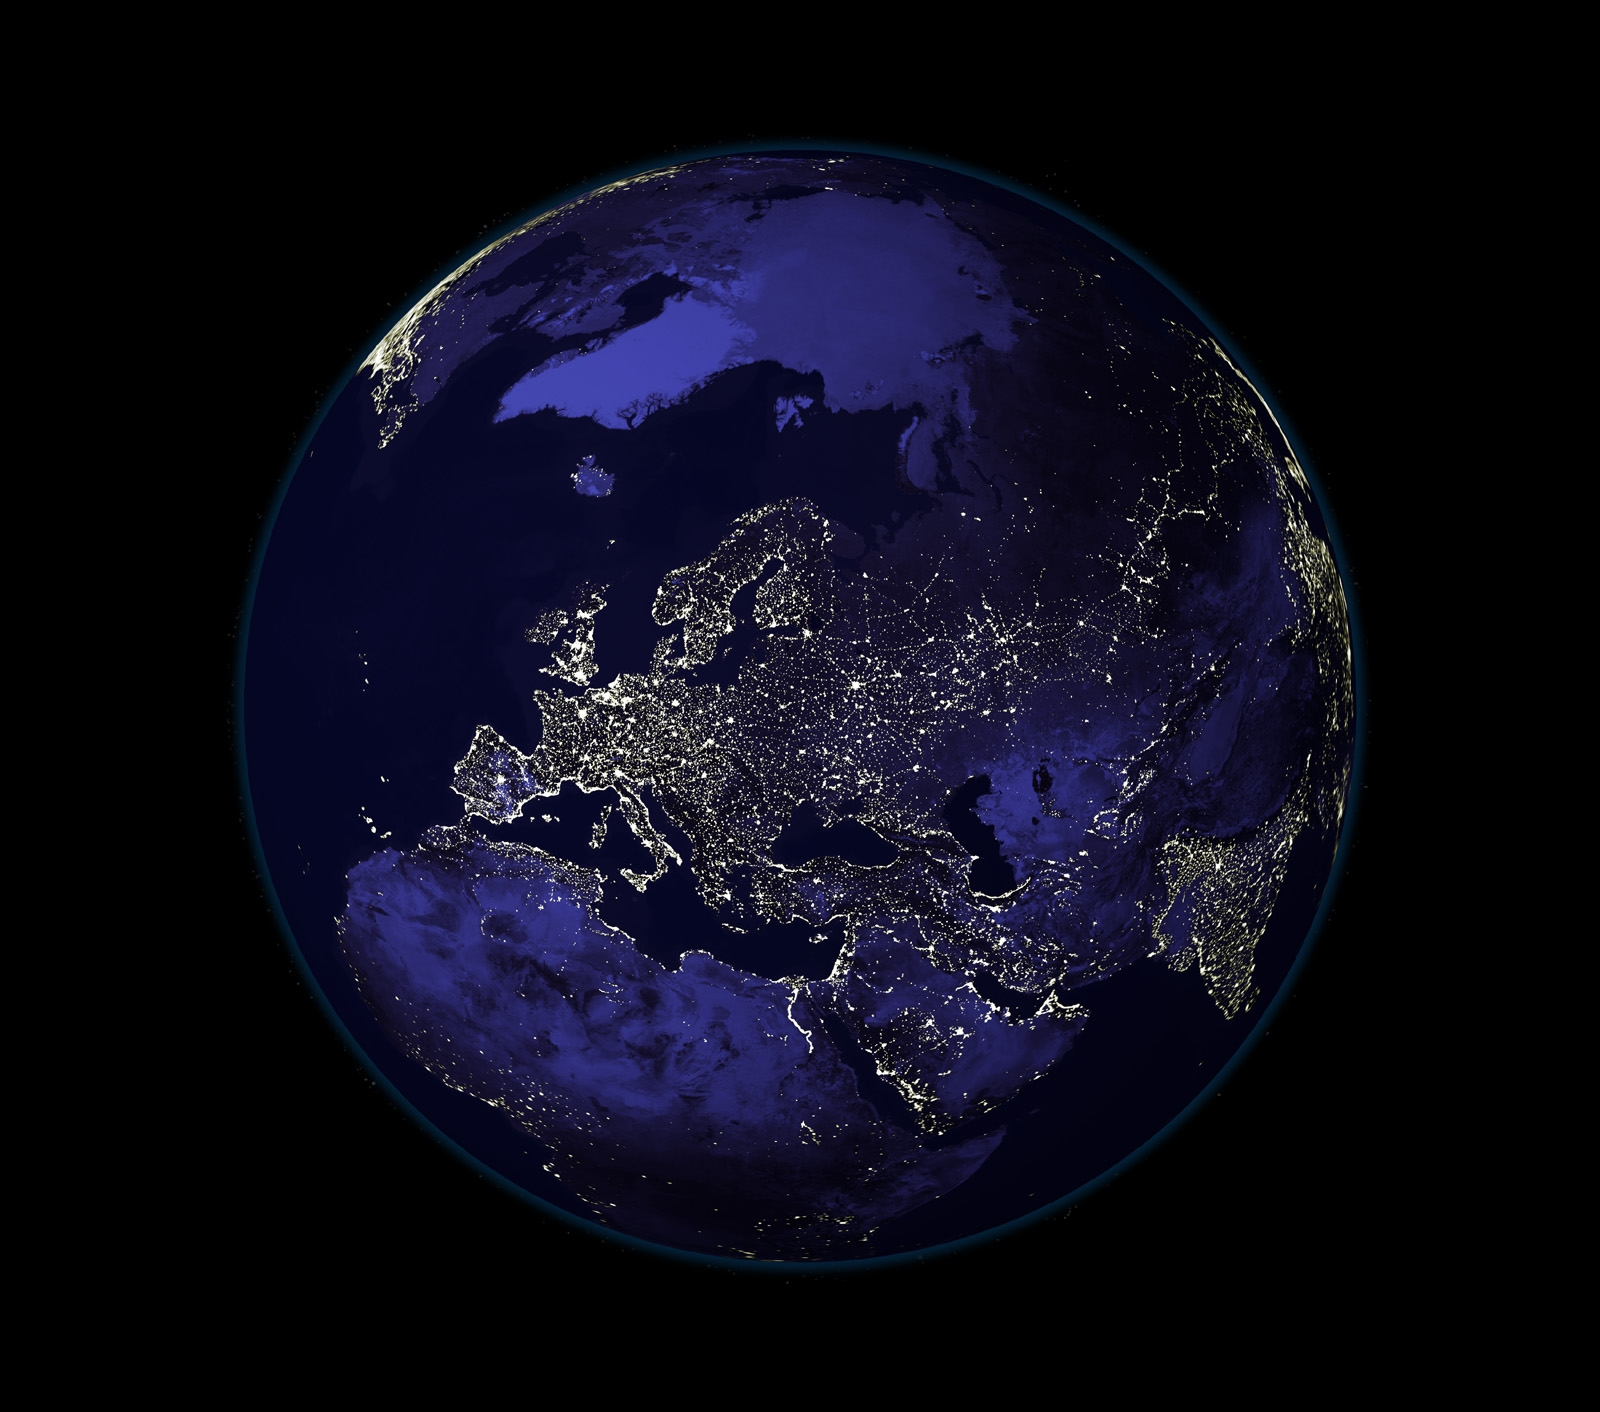
\includegraphics[width=0.5\textwidth]{Tellus}
	\end{center}
\end{figure}

The origin of life problem is really a problem of how that entire process of life gets started in the first place and it's ultimately critically important to the field of astrobiology that we understand that process because we want to know on how many worlds that occurs.


\section{Exoplanets}

\subsection[The Habitable Zone]{The Habitable Zone--Elizabeth Tasker}

This lecture takes us away from our own planet to look at what we currently know about
planets orbiting around other stars.
Before the early 1990s, the only planets we knew for sure that existed were the worlds that orbited around our own Sun, but as our instruments became sensitive enough to spot
the dim whisper of a planet around other stars in our galaxy, we discovered our planetary system was one of multitudes--Figure \ref{fig:exoplants}.


\begin{figure}[H]
	\caption{Exoplanets by discovery technique}\label{fig:exoplants}
	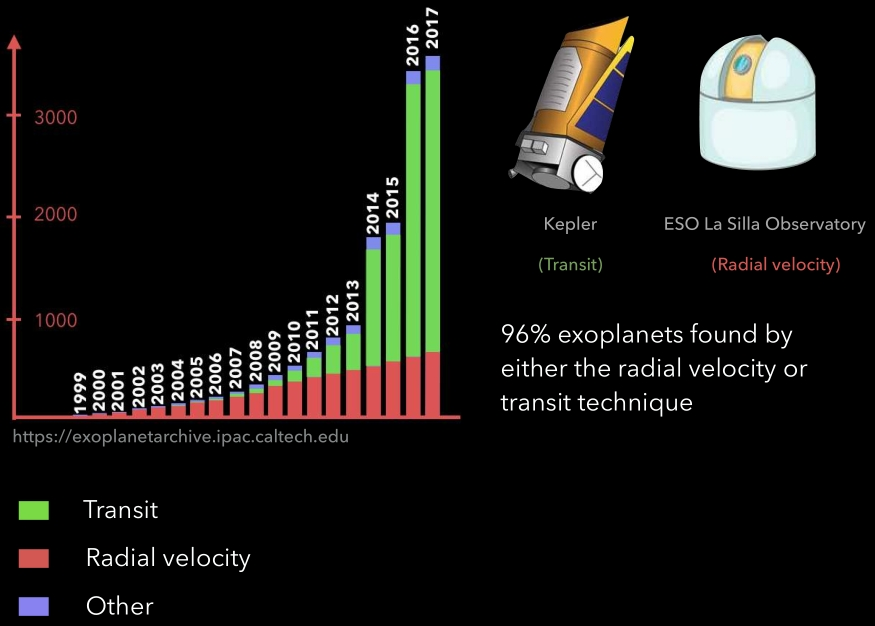
\includegraphics[width=0.9\textwidth]{Exoplanets}
\end{figure}

We now know of thousands of extrasolar planets or exoplanets--planets that orbit stars
other than our Sun.
This results in an obvious question: could any of these newly discovered worlds be habitable?

\begin{figure}[H]
	\caption{Could any of these newly discovered
		worlds be habitable?}\label{fig:could-any-be-habitable}
	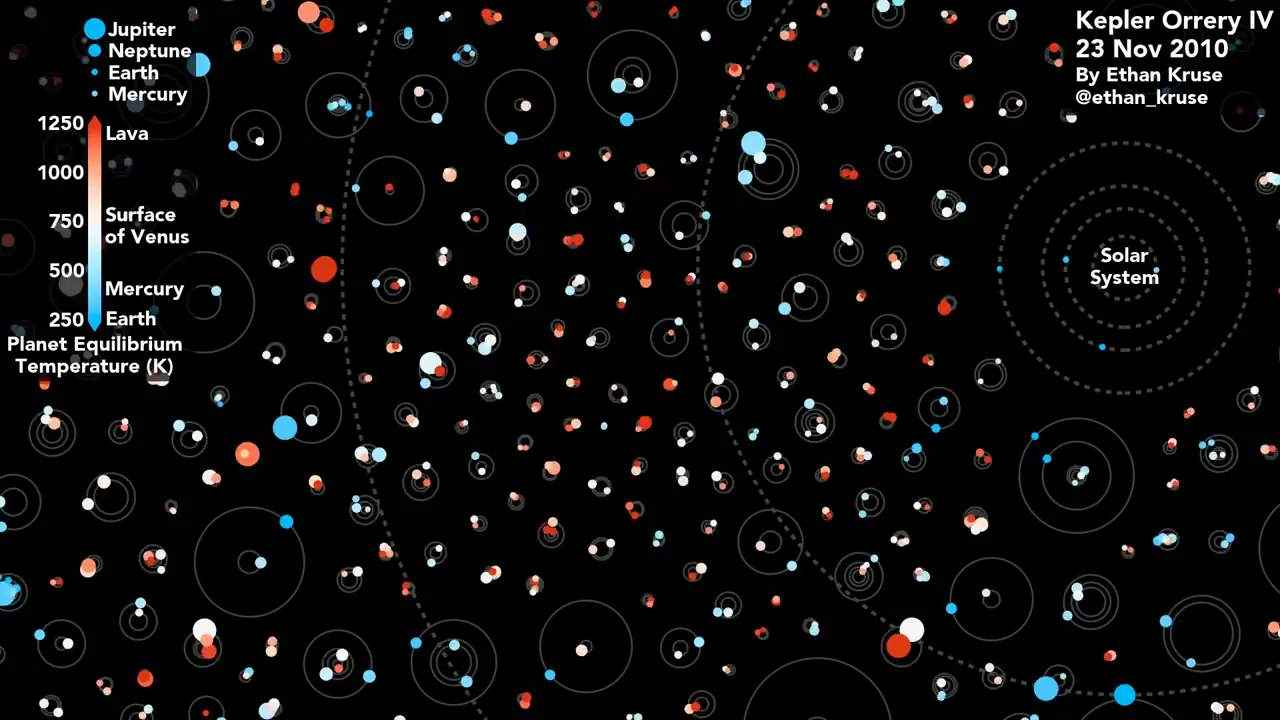
\includegraphics[width=\textwidth]{could-any-be-habitable}
\end{figure}
The problem with that question is, while we have discovered many worlds, we actually know very little about each planet. The majority of planets
we have discovered so far have been found by one of two techniques--Figure \ref{fig:exoplants}:
\begin{enumerate}
	\item the radial velocity technique used by ground-based telescopes, such as the \gls{gls:ESO}  in Chile----Figure \ref{fig:radio-velocity-technique0};
	\item the transit technique used by instruments such as the Kepler space telescope and its successor--\gls{gls:TESS}--Figure \ref{fig:transit}.
\end{enumerate}

\begin{figure}[H]
	\caption[The radial velocity technique]{The radial velocity technique, sometimes known as the "Doppler wobble," detects a planet via the tiny wobble it excites in the star. While we normally think of the star as stationary and the planet in orbit, in truth, both the star and planet orbit their common center of mass--Figure \ref{fig:radio-velocity-technique}. As a star is so much bigger than the planet, this center of mass lies very close to the star's own center, causing its orbit to be just a tiny wobble in comparison to the planet's wide circuit. This wobble causes the star to move periodically slightly further away and then closer to the Earth. As the star moves slightly from the Earth, its light waves stretch out and redden slightly--Figure \ref{fig:radio-velocity-technique1}. Conversely, as a star moves back towards us, the light waves compress and become bluer. This regular shift from red to blue is what astronomers can measure to detect a planet--Figure \ref{fig:radio-velocity-technique2}.}\label{fig:radio-velocity-technique0}
	\begin{subfigure}[t]{0.3\textwidth}
		\caption{The star and planet orbit their common center of mass}\label{fig:radio-velocity-technique}
		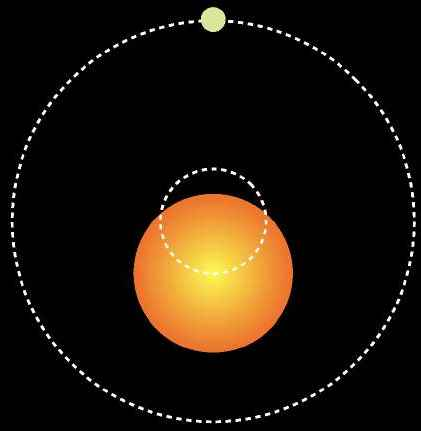
\includegraphics[width=\textwidth]{radio-velocity-technique}
	\end{subfigure}
	\;\;\;
	\begin{subfigure}[t]{0.3\textwidth}
		\caption{As the star moves slightly from the Earth, its light waves stretch out and redden slightly}\label{fig:radio-velocity-technique1}
		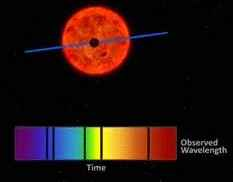
\includegraphics[width=\textwidth]{radio-velocity-technique1}
	\end{subfigure}
	\;\;\;
	\begin{subfigure}[t]{0.3\textwidth}
		\caption{This regular shift from red to blue is what astronomers can measure to detect a planet}\label{fig:radio-velocity-technique2}
		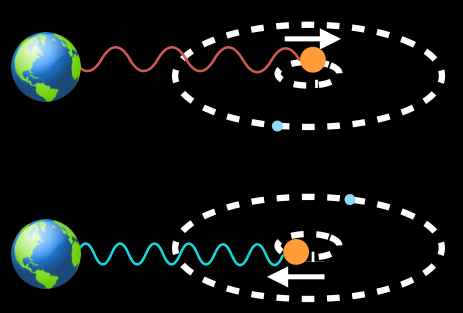
\includegraphics[width=\textwidth]{radio-velocity-technique2}
	\end{subfigure}
\end{figure}

\begin{figure}[H]
	\begin{center}
		\caption[The transit technique]{The second main method for planet detection is the transit technique. Here, a slight dip in the star's brightness is detected as the planet passes in front of the star as seen from Earth.}\label{fig:transit}
		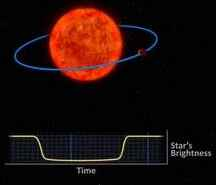
\includegraphics[width=0.5\textwidth]{transit}
	\end{center}
\end{figure}

These two methods give you just two properties about the planet--Figure \ref{fig:planet-properties}.
The transit technique gives you an estimate of the planet's radius while the radial velocity technique tells you about the planet's minimum mass.
This may be significantly less than the true mass of the planets, as the radial velocity technique only measures the wobble of the star directly towards the Earth.
If the planet's orbit is tilted with respect to us, then part of the star's motion
will be directed away from us.
We won't measure this and so will underestimate the planet mass.

\begin{figure}[H]
	\begin{center}
		\caption{These two methods give you just two properties about the planet}\label{fig:planet-properties}
		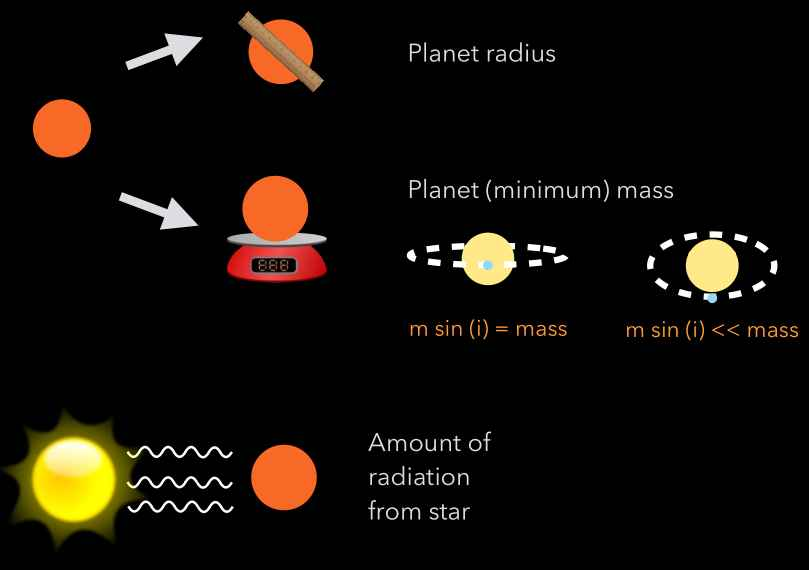
\includegraphics[width=0.8\textwidth]{planet-properties}
	\end{center}
\end{figure}
Both techniques also tell you about the amount of radiation the planet receives from the star.
But, this can be very different from the surface temperature, as it does not allow for
the heat trapping effects of the different atmospheric gases.

The challenge we're trying to determine--if a plant is habitable--is therefore that we can only measure two or three properties and none of these actually tell us what it's like on the planet surface.
This will change as the next generation of telescopes will be able to detect light that passes through the planet's atmosphere.
Different molecules in the atmosphere absorb different wavelengths of light, providing a fingerprint of missing wavelengths that indicate atmospheric composition--our first hint at what is happening on the planet's surface.

But, this brings us to a new problem: such atmospheric spectroscopy for rocky, temperate planets is time-consuming and difficult.
We therefore need a way of selecting planets most likely to reveal interesting results.
But how do we select planets best suited for habitability without knowing any surface properties?

Let's think about what we want to find.
It's going to be easiest to recognize Earth-like life, that is, water and
carbon-based chemistry.
Also, this needs to be detectable, which means the water needs to be on the surface of the planet, not a subsurface system like Europa.

Based on this, we can ask the question: how much \gls{gls:insolation} does an Earth-like planet need?
The answer to this is the \emph{Classical Habitable Zone}--Figure \ref{fig:classical:habitable:zone}.

\begin{figure}[H]
	\caption{Classical Habitable Zone}\label{fig:classical:habitable:zone}
	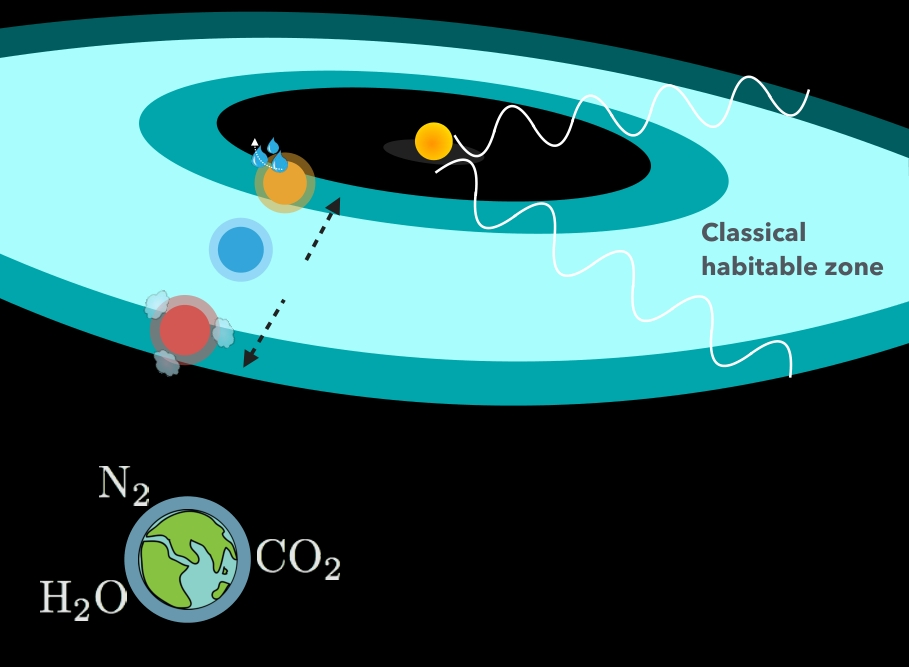
\includegraphics[width=\textwidth]{ClassicalHabitableZone}
\end{figure}

The Classical Habitable Zone is where an Earth-like planet, that is, a planet with our surface pressure, atmospheric gases and geological processes can support water on the surface.
Often, in exoplanet literature, this is simply referred to as the "habitable zone", as we don't yet know about planets other than the Earth that can support life.
At the inner edge of the habitable zone, it is too warm for surface water on the Earth and it evaporates.
At the outer edge, carbon dioxide condenses into clouds and is no longer able to provide
the thermal insulation of a greenhouse gas--so the planet freezes.
Climate models predict that the habitable zone should stretch between 0.99 au and 1.67 au
where 1 au is the average distance of the Earth from the Sun.
Our planet, therefore,sits right on the inner edge.

A slight extension to this is known as the "optimistic habitable zone," which can broaden these limits based on the idea that Venus and Mars probably have
supported surface water in their past--Figure \ref{fig:optimistic:habitable:zone}.

\begin{figure}[H]
	\caption[Optimistic Habitable Zone]{Optimistic Habitable Zone\cite{kasting1993habitable,kopparapu2013habitable}}\label{fig:optimistic:habitable:zone}
	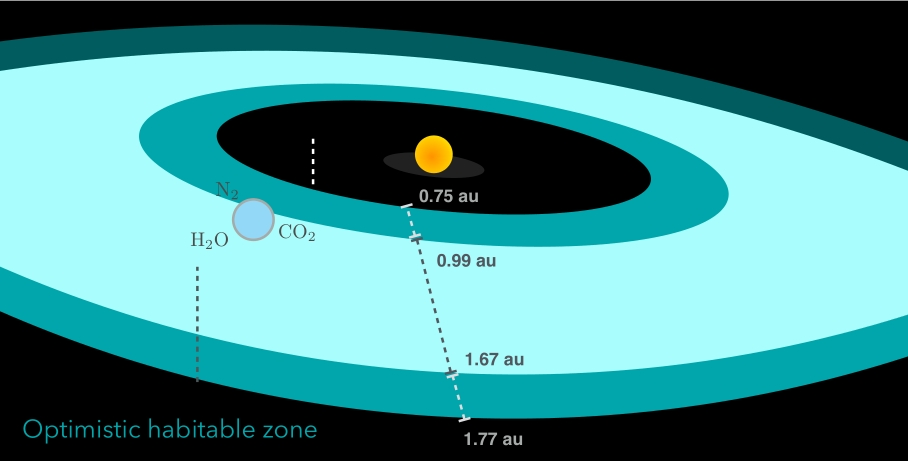
\includegraphics[width=0.9\textwidth]{OptimisticHabitableZone.jpg}
\end{figure}

So, an earth-like planet could have a period of habitability just outside the habitable zone edges.
The edges of the classical habitable zone are only calculated for the Earth.
This is easily demonstrated as, while Venus sits outside the habitable zone, both the Moon and Mars orbit within it but neither are Earth-like enough to support liquid water in this region.
Different planets might have different habitable zones at different locations, or they may not have a habitable zone at all.

Of the planets we have found so far orbiting in the classical habitable zone, almost 15 times as many are large enough to be likely to have thick, Neptune-like atmospheres compared to planets that might be rocky.
We have discovered planets that are the right size to be rocky and orbit entirely within
the habitable zone--Figure \ref{fig:are:these:earthlike}.
Are these Earth-like enough to support liquid water in this region?



We don't know. They may have very different atmospheric gases or geology that makes
surface water impossible. The only thing we can say is that if another habitable,
Earth-like planet is out there, it would be in the habitable zone, but being in the habitable zone does not mean you're Earth-like enough for life.

\begin{figure}[H]
	\begin{center}
		\caption{Are these exoplanets Earth-like?}\label{fig:are:these:earthlike}
		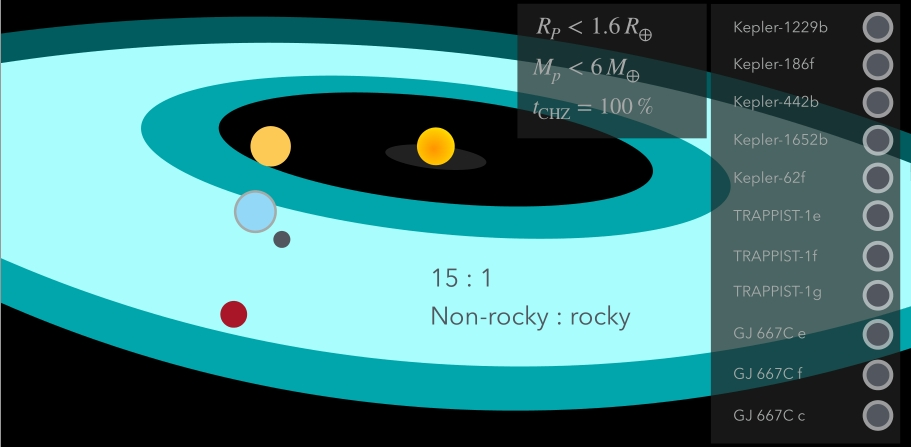
\includegraphics[width=0.9\textwidth]{AreTheseEarthlike}
	\end{center}
\end{figure}

So, in conclusion:\begin{itemize}
	\item  we've discovered thousands of exoplanets, many of which are similar in size to the Earth; 
	\item at the moment, we have no way of knowing what their surfaces are like. Note, in particular, that the Earth and Venus are both very similar in size--so, they are both Earth-sized planets;
	\item our next generation of telescopes will be able to detect the atmosphere of these worlds and tell us something about their surfaces for the first time.
	
	\item the habitable zone is a useful concept for selecting planets for these new telescopes but it offers no guarantee that a planet is actually habitable.
\end{itemize}

References:
\begin{itemize}
	\item If you'd like to try playing with a simple climate model of an Earth-like planet, you can head over to Earthlike World \cite{earthlike.world} or the associated Twitter feed. This website lets you see how different a planet might be from our own world today, even if it did have the same geological cycles as our own.

	\item The NASA \gls{gls:NExSS} "Many Worlds" blog\cite{nexss.info} covers the latest news for exoplanets and many origin of life stories.

	\item There's also a more technical overview of the search for biosignatures in a paper led by Yuka Fujii, published in "Astrobiology" last year--Figure \ref{fujii2018exoplanet}.

	\item See also \cite{villanueva2015unique}.
\end{itemize}

\subsection[Exoplanet Atmospheric Characterization]{Exoplanet Atmospheric Characterization--Yuka Fujii}

Astronomers have discovered
thousands of extrasolar planets
or exoplanets.
Is any of them inhabited like the Earth?
How can we search for it?
In this lecture, I will talk about
the techniques to study exoplanet
atmospheres and possibly surfaces,
which is an essential step towards
finding life on exoplanets.
Detection of exoplanets typically
comes with two properties:
the size and the orbit,
including the distance from the host star--Figure \ref{fig:discovered:exoplanets}.

\begin{figure}[H]
	\caption{Discovered Exoplanets}\label{fig:discovered:exoplanets}
	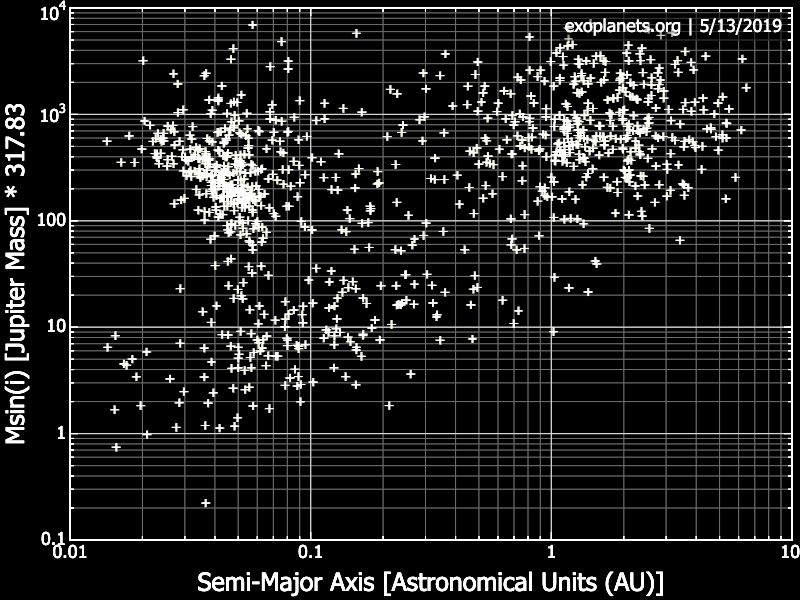
\includegraphics[width=0.9\textwidth]{ExoplanetCharacteristics}
\end{figure} 


For evaluating their potential for life,
we definitely need to get
more information.
But, how?
It has to be reminded that
exoplanets are light-years away.
This means that it's not realistic
to actually visit there
and it's not possible either
to get the spatially resolved images,
unlike the case of solar system planets.
They are just point sources
and we have to rely on remote
observations of these faint dots.
But, observations of these faint dots,
if possible at all,
can in principle give us hints
about the nature of the planets.
For example,
if you observe an Earth Twin--Figure \ref{fig:spectrum:earth:twin0},
Figure \ref{fig:spectrum:earth:twin} shows the overall spectrum
you would get.

\begin{figure}[H]
	\caption{Spectrum of an earth twin}
	\begin{subfigure}[b]{0.3\textwidth}
		\caption{Spectrum of an earth twin}\label{fig:spectrum:earth:twin0}
		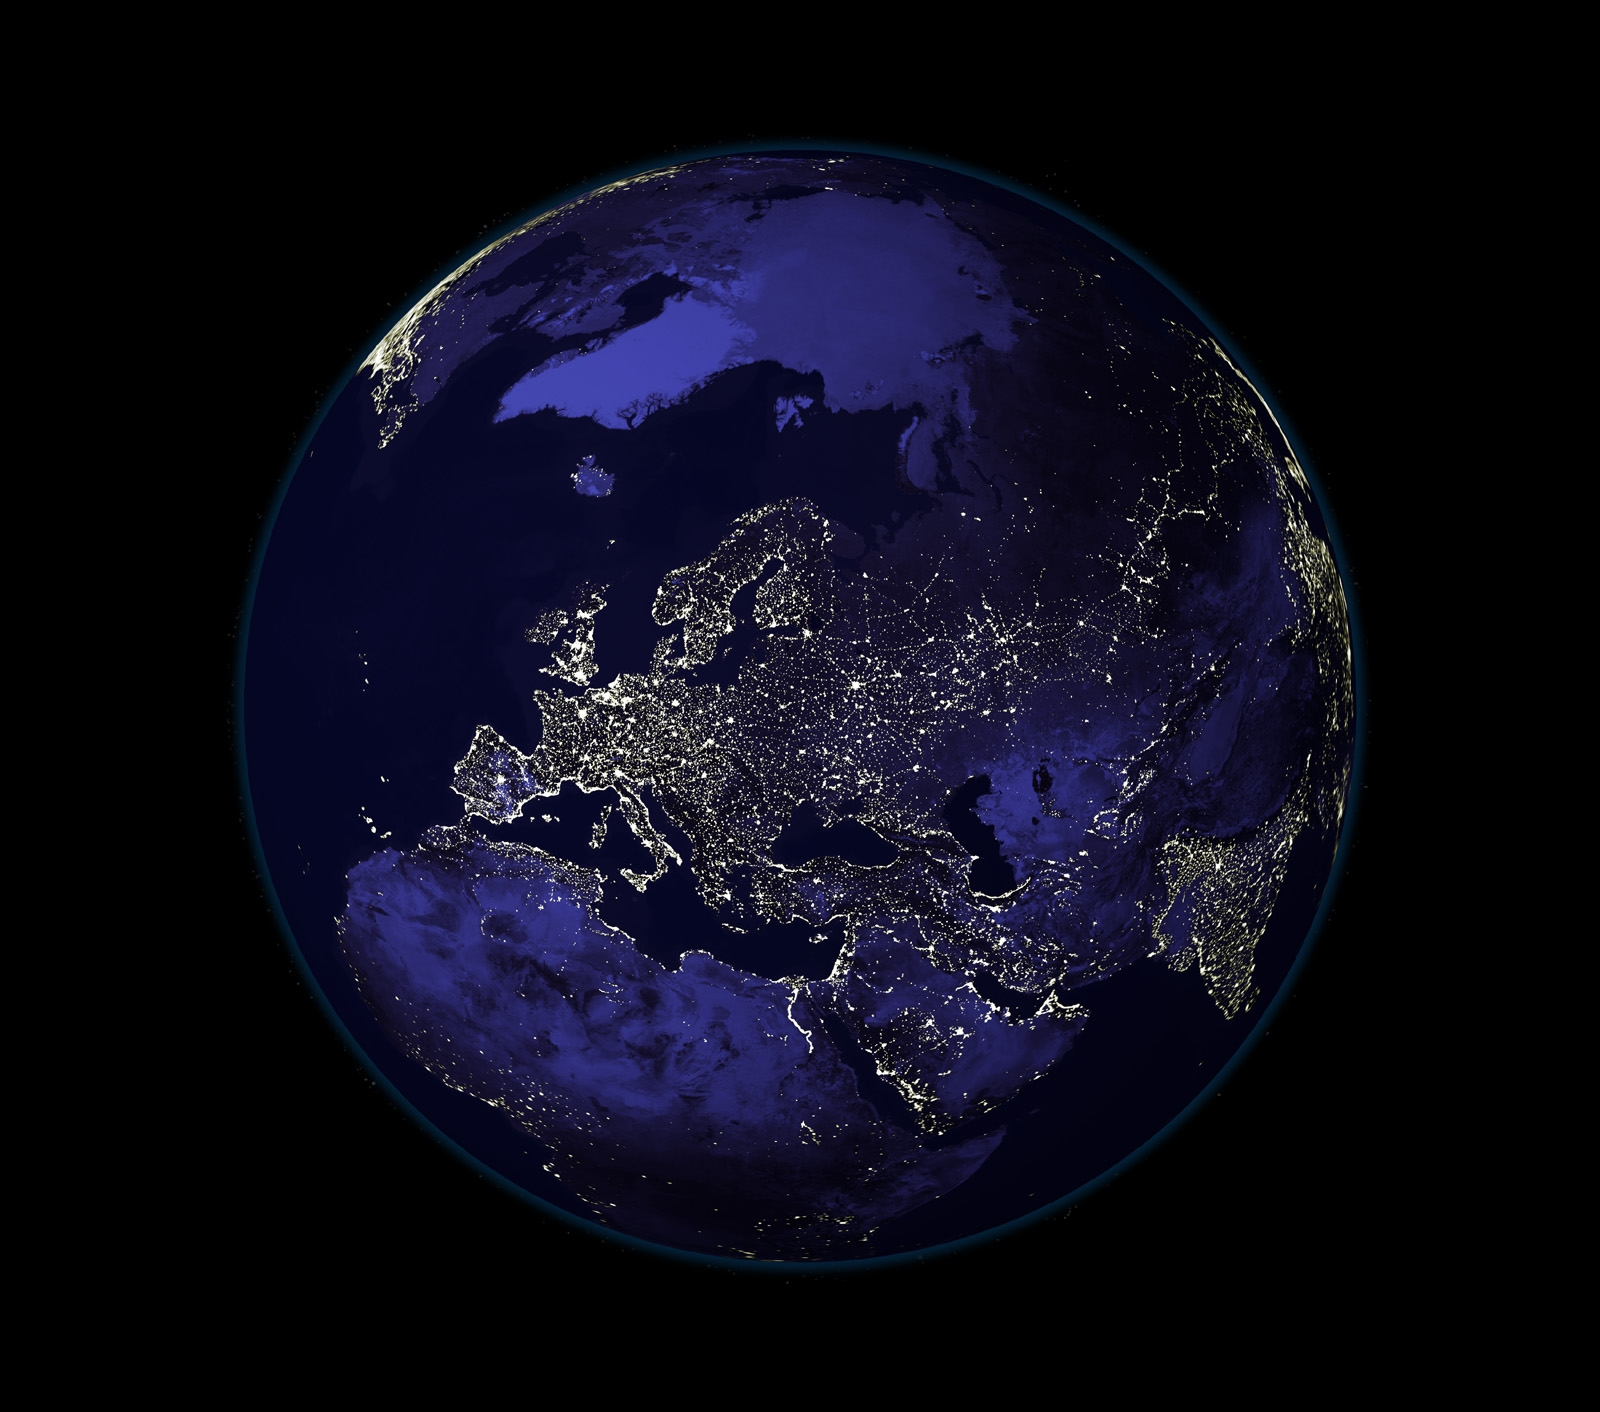
\includegraphics[width=\textwidth]{Tellus}
	\end{subfigure}
	\begin{subfigure}[b]{0.3\textwidth}
		\caption{Spectrum of an earth twin}\label{fig:spectrum:earth:twin}
		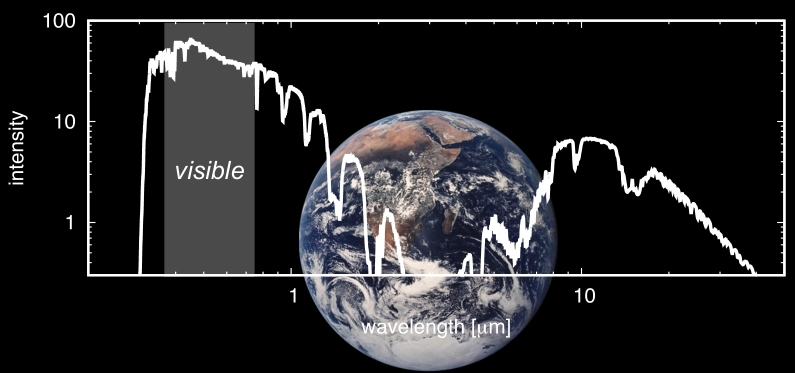
\includegraphics[width=\textwidth]{SpectrumEarthTwin}
	\end{subfigure}
	\begin{subfigure}[b]{0.3\textwidth}
		\caption{At shorter wavelengths the planet scatters light}\label{fig:spectrum:earth:twin1}
		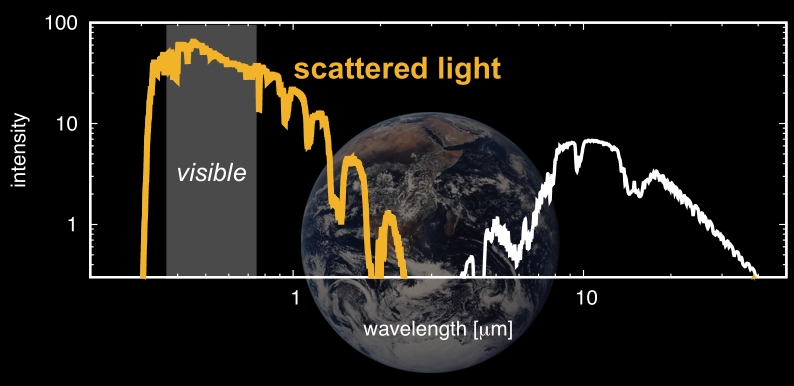
\includegraphics[width=\textwidth]{SpectrumEarthTwin1}
	\end{subfigure}
	\begin{subfigure}[b]{0.45\textwidth}
		\caption{At longer wavelengths it emits infrared}\label{fig:spectrum:earth:twin2}
		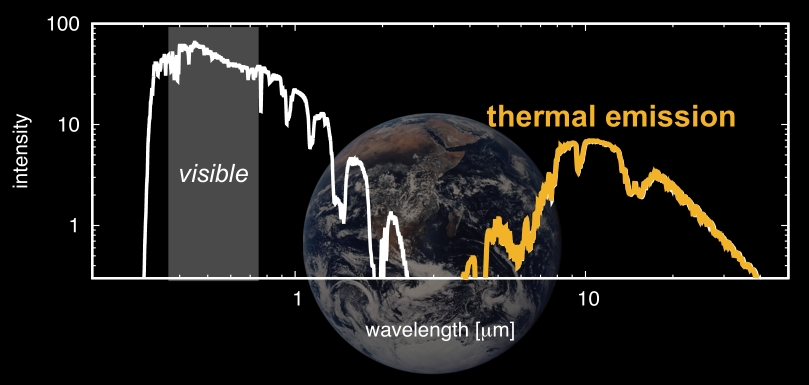
\includegraphics[width=\textwidth]{SpectrumEarthTwin2}
	\end{subfigure}
	\begin{subfigure}[b]{0.45\textwidth}
		\caption{Absorption by atmospheric species}\label{fig:spectrum:earth:twin3}
		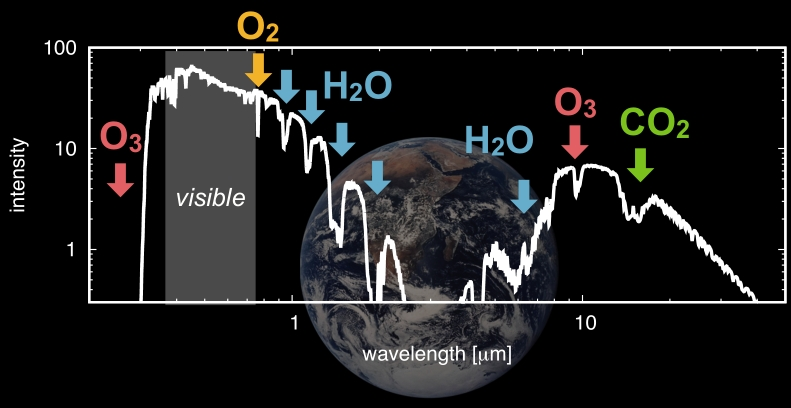
\includegraphics[width=\textwidth]{SpectrumEarthTwin3}
	\end{subfigure}
\end{figure}


At shorter wavelength,
the planet illuminates
by scattering the light
from the host star--Figure \ref{fig:spectrum:earth:twin1}.
And, it's blue features depend on,
for example,
surface composition,
atmospheric pressures and clouds.
On the other hand,
in the invisible infrared range,
the planet emits light
because of its thermal energy--Figure \ref{fig:spectrum:earth:twin2}--
and its baseline depends on
the temperature structure
of the surface layers.
Imprinted in these baselines
are the lower features
due to absorption
by atmospheric species--Figure \ref{fig:spectrum:earth:twin3}.
In the case of an Earth Twin,
they include astrobiologically important
water vapor, oxygen
and ozone features.

We could also potentially use
the time variation of these features
due to planet rotation,
which essentially allows us
to scan the planet
and highlight the regional features.
However, it's not straightforward
to detect the light from exoplanets.
Seen from afar, an exoplanet is
very close to its own host star,
and the star is several to ten
orders of magnitude brighter.
It's equivalent to seeing a firefly
right next to a lighthouse.
Suppose you try to take a picture
of an exoplanet.
Then, the host star is always there,
and, on the imaging plane,
the star is blurred
and the planet is in the skirt of it--Figure \ref{fig:StarIsMuchBrighter}.

\begin{figure}[H]
	\caption[The star is many orders of magnitude brighter than its planets]{Unfortunately the star is many orders of magnitude brighter than its planets}\label{fig:StarIsMuchBrighter}
	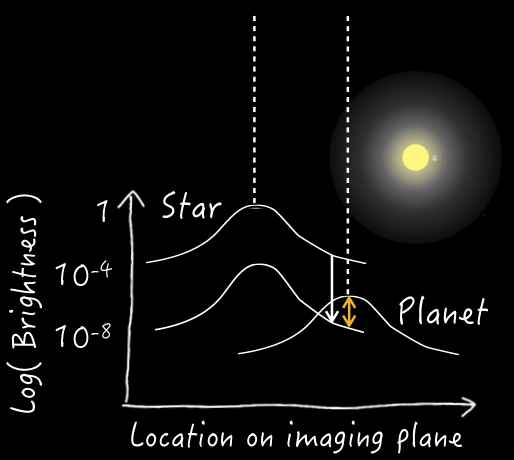
\includegraphics[width=\textwidth]{StarIsMuchBrighter}
\end{figure}

Compared to the peak intensity,
the skirt is orders of magnitude darker,
but planets are often even fainter,
so the signal is varied.
In order to identify the planetary signal,
we need to suppress the light
from the host star
using special instruments.
The idea of such direct imaging
observations of Earth-like planets
dates back to the 1990s.
But, the starlight suppression
is technically challenging.

In the past decade,
direct imaging has been successful
for young, luminous, giant,
gaseous planets at wide orbits--Figure \ref{fig:young:jupiter0}.
Earth-like planets are about
ten times smaller in diameter
and much fainter than
these successful targets.
The efforts are ongoing to achieve
the hyper-suppression level
to be able to detect an Earth Twin.


\begin{figure}[H]
	\caption{Success with Young Jupiter-like Planets in Distant Orbits}\label{fig:young:jupiter}
	\begin{subfigure}[b]{0.25\textwidth}
		\caption{Young Jupiter-like Planet}\label{fig:young:jupiter0}
		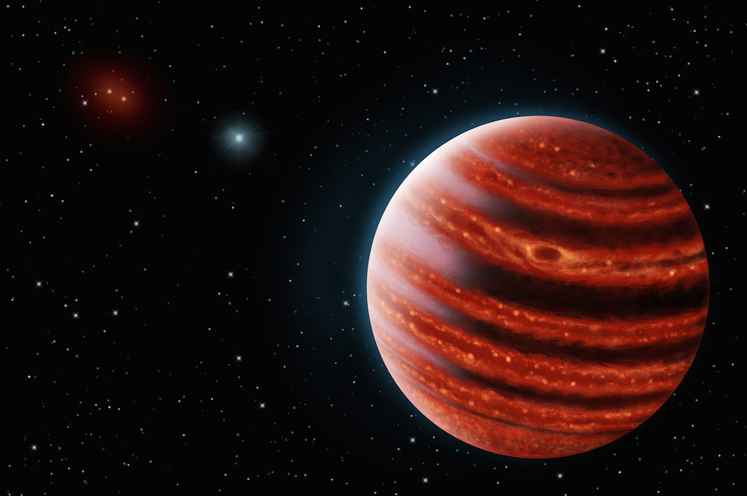
\includegraphics[width=\textwidth]{young-hot-jupiter}
	\end{subfigure}
	\;\;\;
	\begin{subfigure}[b]{0.3\textwidth}
		\caption{ Images of a fourth planet orbiting hr 8799\cite{marois2010images}}\label{fig:young:jupiter1}
		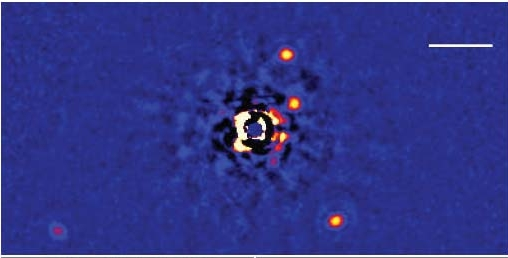
\includegraphics[width=\textwidth]{DirectImaging1.jpg}
	\end{subfigure}
	\;\;\;
	\begin{subfigure}[b]{0.35\textwidth}
		\caption{Gpi spectra of hr 8799 c, d,
			and e\cite{greenbaum2018gpi}}\label{fig:young:jupiter2}
		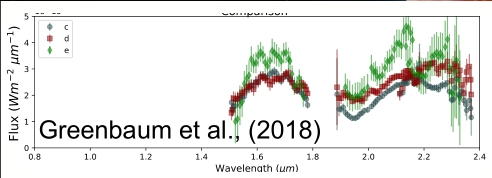
\includegraphics[width=\textwidth]{DirectImaging2.jpg}
	\end{subfigure}
\end{figure}

Meanwhile, the discovery
of transiting planets
opened up new possibilities
to study exoplanet atmospheres
without using special instruments--Figure \ref{fig:transiting:planets}.

\begin{figure}[H]
	\caption[Transiting Planets]{The discovery
		of transiting planets
		opened up new possibilities
		to study exoplanet atmospheres
		without using special instruments}\label{fig:transiting:planets}
	\begin{subfigure}[b]{0.2\textwidth}
		\caption{A transiting planet}\label{fig:transiting:planets1}
		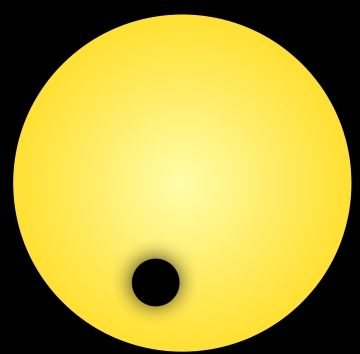
\includegraphics[width=\textwidth]{TransitingPlanets1}
	\end{subfigure}
	\;\;
	\begin{subfigure}[b]{0.3\textwidth}
		\caption{A planet which	passes right in front of the star
			because its orbital plane is close to the line of sight}\label{fig:transiting:planets2}
		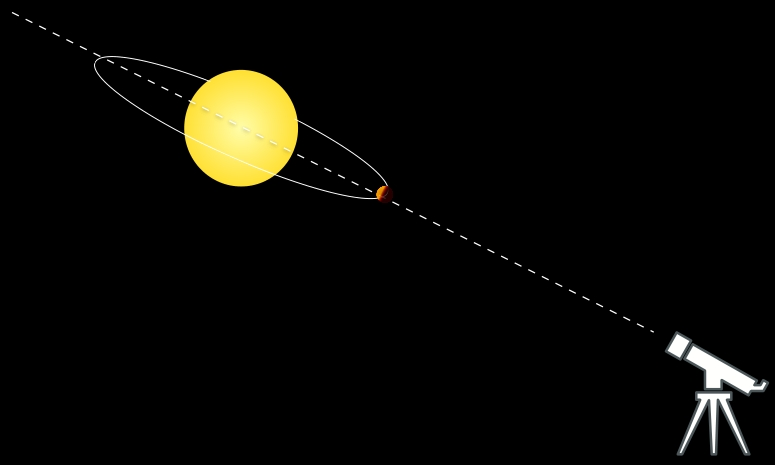
\includegraphics[width=\textwidth]{TransitingPlanets2}
	\end{subfigure}
	\;\;
	\begin{subfigure}[b]{0.31\textwidth}
		\caption{During the transit, a small portion
			of the stellar light
			is filtered through
			the planetary atmosphere}\label{fig:transiting:planets3}
		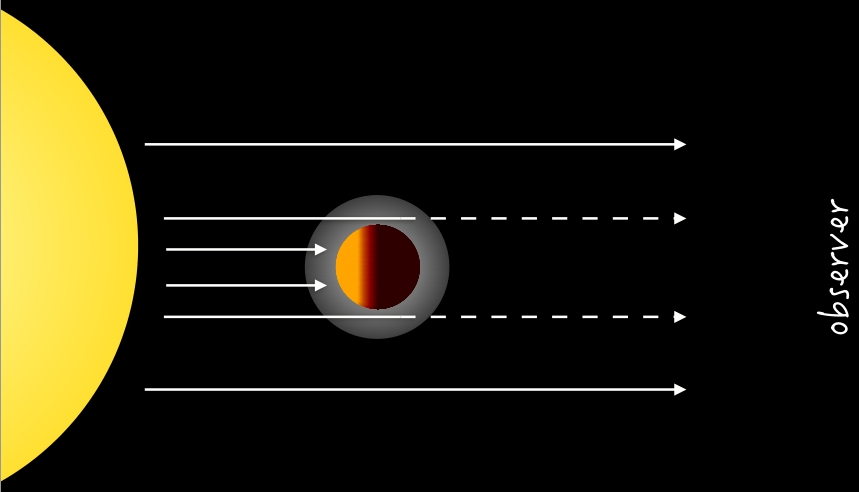
\includegraphics[width=\textwidth]{TransitingPlanets3}
	\end{subfigure}
\end{figure}

A transiting planet is a planet which
passes right in front of the star
because its orbital plane
is close to the line of sight--Figure \ref{fig:transiting:planets2}.
During the transit, a small portion
of the stellar light
is filtered through
the planetary atmosphere--Figure \ref{fig:transiting:planets3}.
By analyzing the spectrum
of this tiny portion
and finding the scattering
or absorption features in there,
we can learn about
the atmospheric composition
and the presence of condensates
such as clouds.
This technique is called
"transmission spectroscopy."

In many cases, transiting planets also pass behind the host star
and that's called "planetary" or "secondary" eclipse--Figure \ref{fig:secondary-eclipse}
\begin{figure}[H]
	\caption{Secondary Eclipse}
	\begin{subfigure}[b]{0.45\textwidth}
		\caption{In many cases, transiting planets also pass behind the host star
			and that's called "planetary" or "secondary" eclipse}\label{fig:secondary-eclipse}
		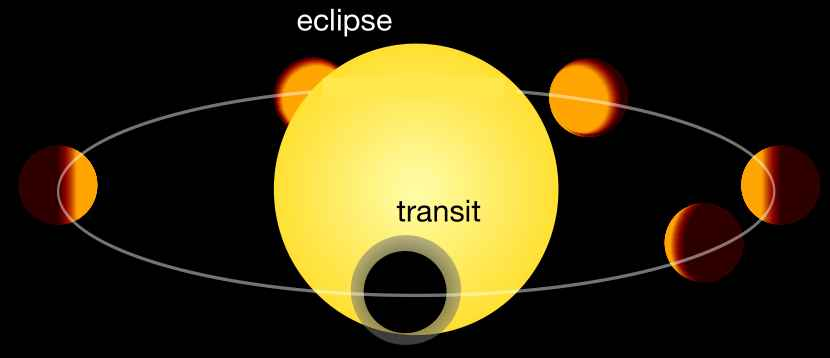
\includegraphics[width=\textwidth]{secondary-eclipse}
	\end{subfigure}
	\begin{subfigure}[b]{0.45\textwidth}
		\caption{The difference between
			the out-of-eclipse total flux
			and the in-eclipse flux
			corresponds to the brightness
			of the planetary dayside}\label{fig:secondary-eclipse1}
		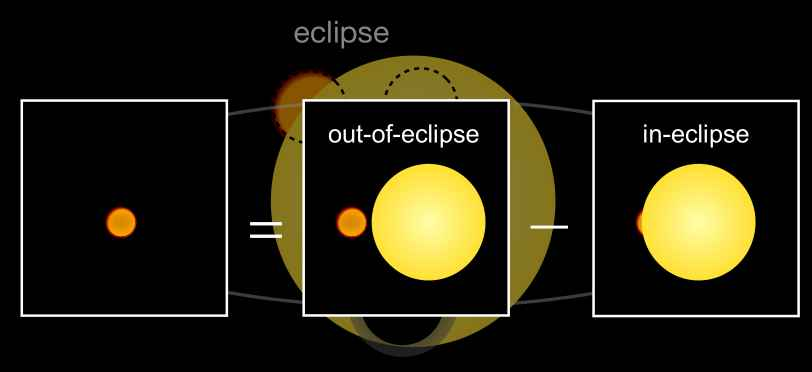
\includegraphics[width=\textwidth]{secondary-eclipse1}
	\end{subfigure}
\end{figure}
At the time of the eclipse,
the planetary flux is blocked by the star.
So, the difference between
the out-of-eclipse total flux
and the in-eclipse flux
corresponds to the brightness
of the planetary dayside--Figure \ref{fig:secondary-eclipse1}.
This way, using planetary eclipse,
we can identify the spectrum
of the planet
without directly separating the star
and the planet in the imaging plate.

In addition, while the planet
orbits the star,
the varying portion of the planetary
dayside faces us
and the planetary flux
changes in time accordingly--Figure \ref{fig:phase-variation}.

\begin{figure}[H]
	\begin{center}
		\caption[Phase Variation]{ while the planet orbits the star, the varying portion of the planetary dayside faces us 	and the planetary flux changes in time accordingly}\label{fig:phase-variation}
		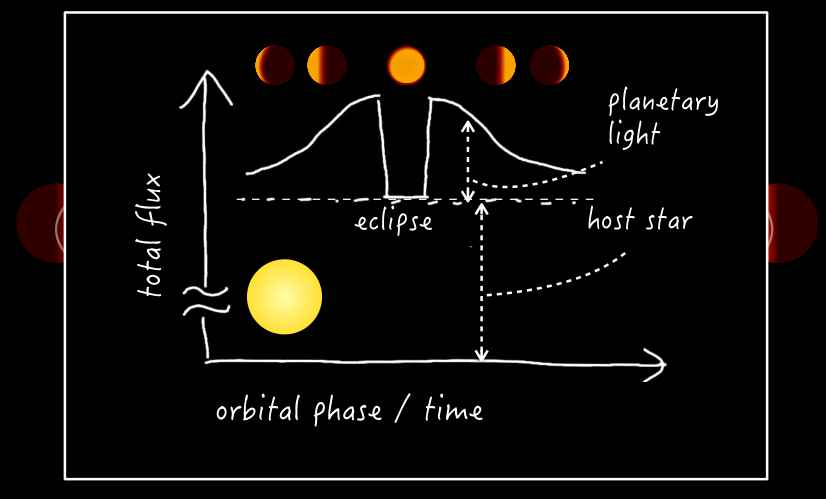
\includegraphics[width=0.8\textwidth]{phase-variation}
	\end{center}
\end{figure}
In turn, although we cannot resolve
the star and the planet,
the time variation in the total flux
can be attributed to
the planetary component
assuming that the star is stable.
These three techniques
have been successful
with hot Jupiter-like planets
and have revealed
some of the atmospheric species
and thermal structures.

In order to apply them to smaller,
potentially habitable planets, however,
we need to push the current
technology to its limit.
The techniques introduced so far
have pros and cons
and the relevant targets vary.
So, we will use all of them
to study various aspects of exoplanets.
In the next decade,
new powerful observatories
with spectroscopic capability
will come into play.
The main targets will probably be
large gaseous planets
but some basic investigations
of terrestrial sized planets
are also being attempted.
Future missions aimed at
the most detailed study
of potentially habitable planets
are currently under discussion.

In this lecture,
we discussed the key observations
to study the nature of exoplanets
beyond their size in the orbit.
I encourage you to think further
about how you would find life
on an Earth Twin light-years away
using these techniques.
It will provide and unique view
on Earth's biosphere.

Summary: Key observations to characterize atmospheres (and surfaces) of exoplanets
\begin{itemize}
	\item Direct Imaging
	\item  Transmission spectroscopy
	\item  Secondary eclipse
	\item  Phase curves
\end{itemize}
Using these techniques, how would you find life on an Earth-twin?


Here are some suggestions for further reading.

\cite{fujii2018exoplanet,sagan1993search,kaltenegger2017characterize,robinson2011earth,deming2013infrared,knutson2007map}

\section[Abstract and general Models for Life]{Abstract and general Models for Life--Sara Imari Walker}

One of the critical questions of
astrobiology is how do we model life;
we can think about abstract or general
models for life. We are
after these because we want to  explain life not
only on earth but also on other
worlds and so we need to come up with as
general a principle as possible. So far a
lot of astrobiology has focused on the
idea of trying to define life, so we have
come up with a lot of different
definitions for life
from numerous different perspectives;Figure \ref{fig:life-word-cloud} is just showing some definitions for life. There are so
many different definitions for life that
has really become quite a muddle as to
how we should be thinking about it in a
more rigorous way.

\begin{figure}[H]
	\begin{center}
		\caption[Life from numerous different perspectives]{Life from numerous different perspectives\cite{trifonov2011vocabulary}}\label{fig:life-word-cloud}
		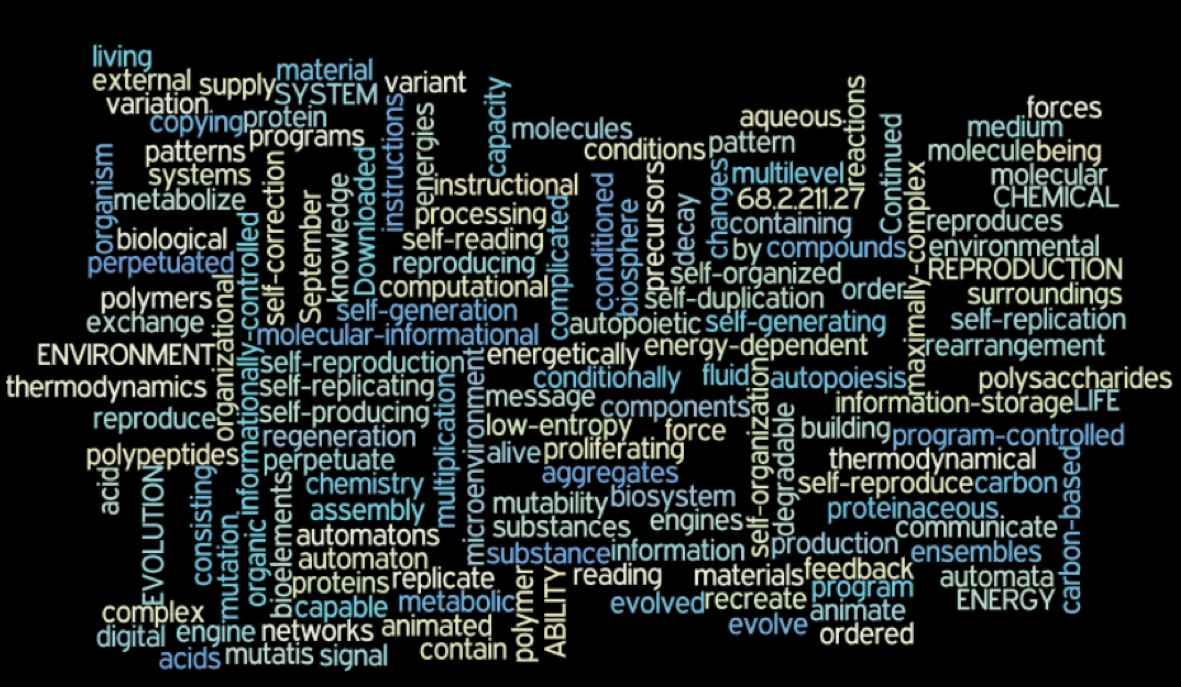
\includegraphics[width=0.8\textwidth]{life-word-cloud}
	\end{center}
\end{figure}

One of the things that  you think about as an astrobiologist is: what's the value of a definition versus a theory or model? A lot of the traditional literature and origins of life has been focused on this idea of defining life so that we can actually be able to identify life on other worlds. The definitions for life are really rather ad-hoc and in
some sense they're  from observations of life on Earth:
\begin{itemize}
	\item  for example we know that life on Earth evolved so we might have an evolutionary definition of life;
	\item or we know that life on Earth is cellular so we might assume that all life requires cells.
\end{itemize}

What we ultimately really need to be aiming for
in the field of astrobiology is to build
better models and theories which might
be more general and allow us to move
beyond definitions of life that are
anthropocentric but
actually become predictive theories for
how life might look on other worlds.

The challenge that we face with anything
trying to get beyond an anthropocentric
or human-centered or earth-centered
viewpoint is that we only have a single
example of life on Earth; despite all
the diversity of life forms that we see--
trees, cats, people bacteria in your gut--
all of that life is related by a common ancestry.
The way that astrobiologists talk
about that is to talk about
the \gls{gls:LUCA}.
If we look at the tree of life
as shown in Figure \ref{fig:yatol}, and we trace
the evolution of all the life-forms that
exist today backwards in time they all
converge on \gls{gls:LUCA}, which is a
\emph{population} of cells that lived on the
primitive earth.


\begin{figure}[H]
	\caption{We are limited by a single example of life}\label{fig:yatol}
	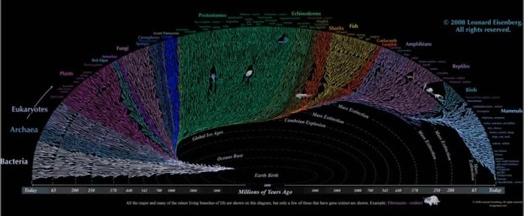
\includegraphics[width=\textwidth]{YATOL}
\end{figure}

We think that all modern life descended from \gls{gls:LUCA}, and the properties that that life-form would have had would have been DNA\footnote{But see \cite{glansdorff2008last} for an RNA world \gls{gls:LUCA}}, and a translation machinery, proteins and cellular architecture much like a modern cell; it was actually a very advanced life-form. It doesn't take us all the way back to the origins of life on earth.
The fact that all life shares this kind of common biochemical architecture is actually really limiting, because it means that we only have one example of life to go on, and extrapolating any kind of general principles from one example is actually rather hard.

What people have done traditionally in the origin of life field is to try to come up with
models that are based on the core components of that architecture of life
that we know today. Two of those core components that have been dominant models for origins of life are what are called genetics first  and metabolism first--Figure \ref{fig:GeneticsVsMetabolism}.

\begin{figure}[H]
	\caption[Genetics-First versus Metabolism-First]{Genetics-First versus Metabolism-First: Two competing hypotheses}\label{fig:GeneticsVsMetabolism}
	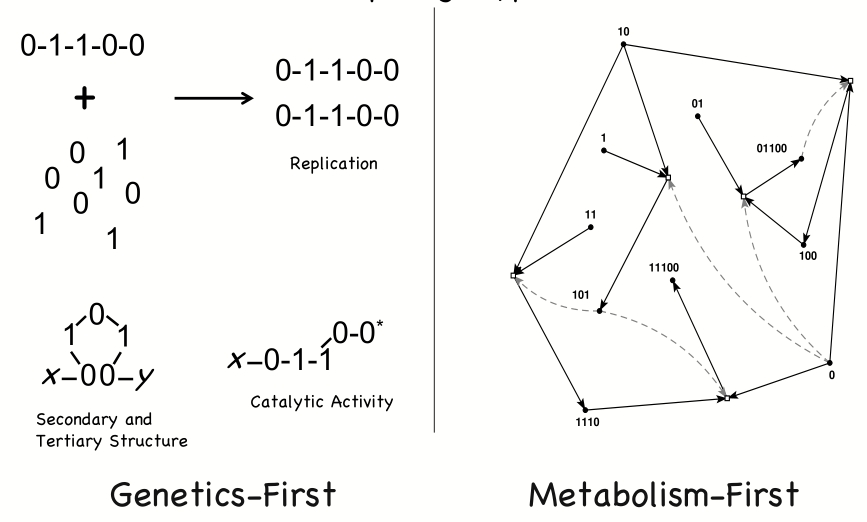
\includegraphics[width=0.9\textwidth]{GeneticsVsMetabolism}
\end{figure}

We know that cells metabolize: they need to acquire food from their environment; you and I need to acquire food in order to survive to reproduce, so metabolism is obviously a
critical component. 
In the genetics first view we also know that life requires genetic information in order to be able to reproduce and to evolve over many generations, so if you split these two kinds of core components of biology to just what that essential thing is we have this sort of genetics idea where people have proposed that the first living entities might have just been molecules like RNA that could copy themselves.
 Figure \ref{fig:GeneticsVsMetabolism} shows an
abstract model, a process
where you might just talk about the the
binary digits in a sequence if it was an
RNA molecule; it would be the sequence of
ribonucleotides in the actual RNA so
that actual basis and you can actually
talk about reproducing that information
via copying.

The RNA world
has been a popular idea because
RNA also has a catalytic function
associated with it, whereas in modern
organisms we have DNA and protein.
DNA controls genetic heredity and
proteins are primarily the catalysts
that actually execute reactions in the
cell, but RNA can do both those functions, so
genetics first has emerged of this idea
that you can model quite simply with
these kind of models where you talk
about copying and heredity and this idea
of evolution through this kind of
process as the core thing that emerged
first as a first living entity.

The metabolism first perspective is an
alternative view that the first kinds of
living entities were not individual
molecules that could replicate but sets
of molecules that were reacting together
and could collectively reproduce due to
the organizational patterns of their
reactions. That idea is called
\gls{gls:autocatalytic:set} theory.
  Figure \ref{fig:GeneticsVsMetabolism} shows
an example of catalytic
sets, using that same kind of
representation  molecules
as binary strings--just strings of zeros
and ones which is a way of modeling
these kinds of processes in artificial
chemistries. In this metabolism-first view the first kinds of living
systems would have been these organized
patterns of chemical reactions.

Both of these perspectives allow one to
model certain attributes of living
systems. But it's really nice if you
actually put them side-by-side and look
at something like the binary polymer
representation of them, because you start
to see that both of them are different
ways of propagating information in
chemical systems; a theme starts to
emerge about what kinds of theories
might unify different approaches to
origins of life. This gets back to
the idea that what we need to start
doing to move forward in origins of life
(whereas traditionally we've had these
models like genetics first, metabolism
first, and there's other models like
compartment first, where
we're talking about
mineral surfaces and all kinds of
things) is to start
thinking about what are the theories for
life, and how do we actually develop more
predictive models that are more generic
to different chemistries and allow us
to actually go to the lab and predict
under what circumstances we should start
getting things that look more lifelike.

And a nice example of the need for
theories and thinking about origins of
life was given by Carol Cleland and
Chris Chyba \cite{cleland2002defining} who talked about
trying to define water and how difficult
it was to actually define water before
we had a molecular theory for water.
You might describe water as a clear
liquid, you might describe it based on
the fact that it's liquid at a certain
range of temperatures, that it 
doesn't have a strong odour; there's a lot
of different ways that you could
describe what water that might lead to a
definition of water but none of them are
really exclusive to water because
there's other clear liquids that you
might describe there's other things that
are also a liquid at room temperature.
The way that we really precisely
define  water is actually to have
an atomic theory that describes
molecules and their interactions; and we
can precisely define water now as $H_2O$.
Their thought was that what we do
now is  phenomenologically define
life, we have a lot of heuristics or a
lot of ideas about what we think life
might be but ultimately what we need is
a theory and that our definition should
derive from the theory not the other way
around.

And one way I like to think about
that is actually to think about like the
emergent\footnote{See glossary entry \gls{gls:emergence}} properties of life.
For example, one of the defining properties
of water has is that it's wet,
but wetness of water is an emergent
property: it requires many many many
millions of water molecules potentially
to be wet (although there's
actually an active debate
about how many water molecules
--if it's a few hundred, a few
thousand--and people have been working to
develop models to quantify when water
gets wet).

Likewise, if we're thinking about
emergent properties of life evolution is
often considered to be a defining
property of life, but evolution exists at
the level of population. It requires
many interacting individuals
in order to be an evolutionary
system, so in some sense evolution,
which we use as a defining property of
life, is also an emergent property of
life; one of the things that we
really need to challenge ourselves with
is to try to find the underlying theory
that explains that emergent property in
the same way that we have an atomic
theory for water that explains some of
its emergent properties.

One of the ways that we might think about that
is life as an
information processing system--Figure \ref{fig:nurse-information}.

\begin{figure}[H]
	\begin{center}
		\caption[Life as an information processing system]{Life as an information processing system\cite{nurse2008life}}\label{fig:nurse-information}
		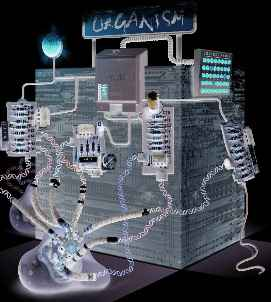
\includegraphics[width=0.6\textwidth]{nurse-information}
	\end{center}
\end{figure}


This is a newer proposal about trying to unify different properties of life;  a lot of people have been very enthusiastic about it in the field, and working on from different perspectives. If we go back to thinking about that genetics versus metabolism picture and we had the binary polymer model, we see they were both a representing an informational system that was capable of reproducing itself; they were just very different architectures for that kind of thing and one might think of genetics first as a
digital type of information processing and metabolism first as an analogue type of information processing. There is this idea in the biological community and also emerging in astrobiology about information possibly being a unifying principle for how we
should think about life across all scales.  Maybe organisms are really organized by flows of information.
One way to think about the origin of life--potentially as kind of a new perspective--is to think about it as a transition and how information is stored propagated and used; this might be sufficiently general to be able to predict properties of alien chemistries
that can also process information in a similar way potentially to Earth's biology but might allow different chemistries than that biochemical architecture that we have on earth as characteristic of \gls{gls:LUCA}--Figure \ref{fig:LifeInformation}.
\begin{quotation}
	Focusing on information… may perhaps provide our best shot at uncovering universal laws of life that work not just for biological systems with known chemistry but also for putative artificial and alien life--\cite{cronin2016beyond}.
\end{quotation}

\begin{figure}[H]
	\caption[Life as Information]{Life as Information\cite{cronin2016beyond}}\label{fig:LifeInformation}
	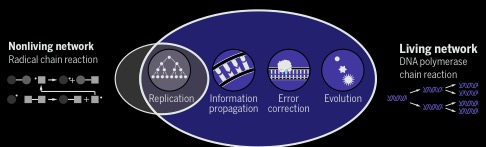
\includegraphics[width=0.9\textwidth]{LifeInformation}
\end{figure}


If we could understand how information works in biochemical networks on earth we could potentially understand what other possible chemistries could enable those same kinds of emergent properties on other worlds and maybe predict alien chemistries

\section[The Multiple Origins of Life]{The Multiple Origins of Life--David Krakauer}

I'm going to talk about the multiple origins of life in complex time. Most people would say life evolved perhaps once, between 3.5 and 4 billion years ago, and the evidence of that evolution are things like fosssilized microorganisms and those organisms are presumed to posses certain key properties. Autocatalylis, replication, metabolism and the ability to adapt. And this is a chemical material theory for the origin of life, and I'm going to say there's another one that's quite distinct that's based on information theory. And here's the argument

\subsection{The Argument}

Origin of Life is dominated by what we would call naturalist reductionistic perspectives. That is, the ultimate understanding of why a system works is an analysis of the chemistry of the most basic building blocks that make up the phenomenon of interest. There's another school called functionalists, who say that those building blocks are necessary but not sufficient. What we really care about are their properties and those properties can be realized in multiple different ways. 

I'm going to make this argument very clear by showing your an analogous argument in the field of artificial intelligence. The idea here is that life emerges from an adaptive arrow of time--Section \ref{section:adaptive}, which is the reverse of the thermodynamic arrow of time that leads to increasing disorder--Section \ref{section:reversing}. And the interesting thing about the adaptive order of time is it's multi scale, rather like the physical arrow of time, meaning it can be be observed at molecular levels all the way through to the scale of whole societies and in that respect, it's not critically dependant on biology or chemistry. And the key to understanding the adaptive arrow of of time is understanding the adaptive agent. The agent is the key concept or sometimes called the individual in complex adaptive systems. And an agent can be a virus, the agent can even be a language. So here is the analogous debate in artificial intelligence.

John Searle is a proponent of biological naturalism. His proposition is that the only system that can be intelligent is a biological one. And he said: \begin{quotation}
	My car and my adding machine 	understand nothing: they are not in that line of business.
\end{quotation} That is you could never build a mechanical device with understanding because they're not made of neurons. In contrast Alan Turing said 	\begin{quotation}
We are not interested in the fact that the brain has the consistency of cold porridge
\end{quotation}, i.e. the materials do not matter as much as we have assumed because we can instantiate function in a range of very different materials. And this argument for intelligence generalizes two arguments about life:
\begin{itemize}
	\item we don't necessarily need the chemistry we have in existing living systems;
	\item there might be very different ways of achieving life like properties.
\end{itemize}



\subsection{Reversing the Arrow of Time}\label{section:reversing}

The key to understanding a functionalist perspective on the origin of life
is understanding the adaptive arrow of time.
If I were to show you this slide--Figure \ref{fig:apples}--and ask you: ''which
way does time flow, from left to right
or right to left? from the fresh to rotten or
rotten to fresh?''-- everyone would know the
answer to that. That's because you have
a basic intuition about the second law of thermodynamics.
Systems tend to become disordered in time.

\begin{figure}[H]
	\begin{center}
		\caption{Which way does time flow, from left to right or right to left?}\label{fig:apples}
		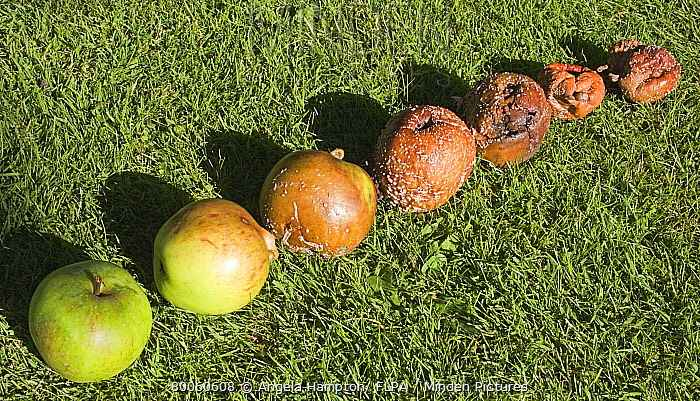
\includegraphics[width=0.8\textwidth]{apples}
	\end{center}
\end{figure}
Arthur Eddington famously described this phenomenon
the arrow of time, by asking us to consider
an arrow and if we follow that arrow and
find more and more of the random element
in the state of the world, then that
points towards the future. But if the
random element decreases, the arrow points
towards the past. And "time's arrow"
expresses the one-way property of time.
\begin{quotation}
	Let us draw an arrow arbitrarily. If as we follow the arrow we find more and more
	of the random element in the state of the world, then the arrow is pointing towards
	the future; if the random element decreases the arrow points towards the past … I
	shall use the phrase “time's arrow” to express this one-way property of time which
	has no analogue in space--Sir Arthur Eddington.
\end{quotation}
Now, most of you are thinking, ''wait a second,
there is a forward arrow that leads
to greater order'', and that's what Darwin
worked on. And so, if I showed you this picture--Figure \ref{fig:butterflies}--
and said, ''which is the initial state and
which is the final state?'', those of you
familiar with the phenomena of industrial melanism
in Northern England, would say, ''well, the final
state here is the adaptive state''. Its the dark
moth with the dark background which is less susceptible to predators.

\begin{figure}[H]
	\begin{center}
		\caption{Butterflies and Time's Arrow}\label{fig:butterflies}
		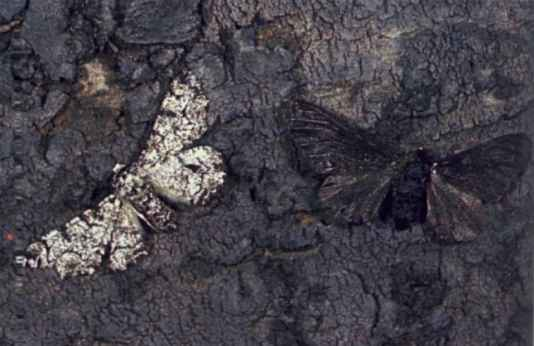
\includegraphics[width=0.8\textwidth]{butterflies}
	\end{center}
\end{figure}

Ronald Fisher expressed this alternative to Eddington's arrow of time as Darwinian arrow
of time, when he said: 
\begin{quotation}
	It was Darwin's chief contribution not only biology but of the whole natural science to have brought to light a process by which randomness that you start with, in the process of time decreases, such that very improbable things their non-occurrence becomes highly probable\cite{huxley1954evolution}.
\end{quotation}

So, the Darwinian arrow of time, rather than increasing probable things--disorder--increases improbable things.
And the standard framework for understanding this increase in improbable things is evolution by natural selection on fitness landscapes--Figure \ref{fig:NaturalSelection}. So there are many probable states of the world, and they are all low-fitness. But there is one high-fitness state of the world, which in terms of of the space of possibilities, is highly improbable.
And, that's what natural selection does. It selects more of these possible states
a very improbable one. And, so the physical arrow of time says you are going to roll down-hill and end up in one of these more probable states and the adaptive arrow of time says you are going move uphill and end up in a very improbable ordered state.

\begin{figure}[H]
	\caption[Thermodynamic Arrow of Time versus Adaptive ]{Thermodynamic Arrow of Time wants to roll down hill, Adaptive up hill towards lower probability.}\label{fig:NaturalSelection}
	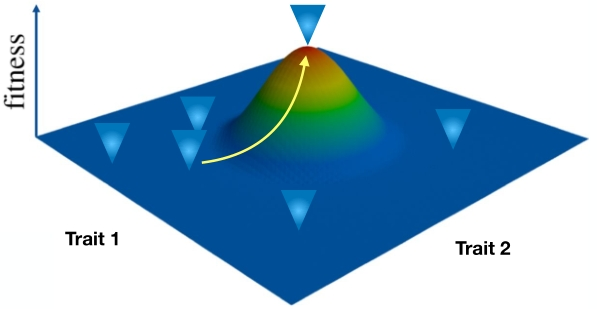
\includegraphics[width=0.9\textwidth]{NaturalSelection}
\end{figure}

\subsection{The Theory of the Adaptive Arrow of Time}\label{section:adaptive}

The adaptive arrow of time tells you that you go
from probable states to an improbable state,
from disordered states to an ordered state.
It is the reverse of the thermodynamic arrow of time.
There have been several efforts to mathematize that fact,
most famously by Ronald A. Fisher
in the so called 'Fundamental Theory of Natural Selection'.

Fisher wanted a theory as general as the second law of thermodynamics.
And here it is, captured in mathematical terms:
It says, you move through a space of possible solutions
in such a way that you minimize the variability in the population.
That is like minimizing the uncertainty.
And at a certain point you reach the maximum
and then there is only one solution that you observe
and that is the one we typically would call 'best adapted'.

There is a problem with the theory,
and that is: it is not completely general.
Think about a situation like this--Figure \ref{fig:rockpaperscissors},
the rock, paper, scissors game
and ask: what is the maximally adapted solution?

\begin{figure}[H]
	\caption{Rock, paper, scissors}\label{fig:rockpaperscissors}
	\begin{subfigure}[t]{0.3\textwidth}
		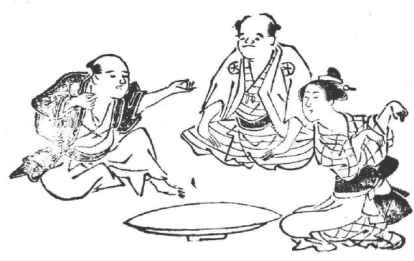
\includegraphics[width=\textwidth]{rockpaperscissors}
	\end{subfigure}
	\begin{subfigure}[t]{0.3\textwidth}
		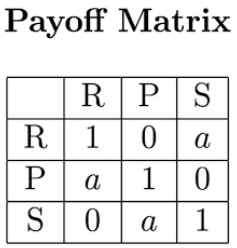
\includegraphics[width=\textwidth]{rockpaperscissors-payoff}
	\end{subfigure}
	\begin{subfigure}[t]{0.3\textwidth}
		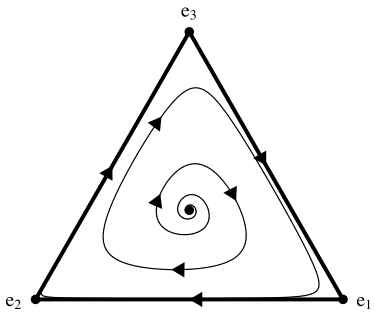
\includegraphics[width=\textwidth]{rockpaperscissors-evolution}
	\end{subfigure}
\end{figure}
Well, imagine that Fisher's fundamental theory was right
you would say that only one of those strategies at the end is where you end up
because you have minimized the variability.
So I always play 'rock'.
But, of course, someone can come along and play paper and beat me.
So, in this particular instance of frequency dependent selection
Fisher's fundamental theory cannot be right,
because you are not minimizing the variance
you are actually maximizing it.

Over the last decade or so a number of us have been working on generalizing the adaptive arrow of time, mathematically, to ask: what is actually being minimized?
All adaptive processes are minimizing
the uncertainty of an agent about the state of the world. Or, put differently, each agent maximizes the amount of information it possesses about the world in which it lives.
And when you express the adaptive arrow of time in these terms,
you realize that a whole range of apparently distinct phenomena
- evolution, Bayesian inference, reinforcement learning -
are all examples of the same fundamental dynamic--Figure \ref{fig:evolution-inference-learning}
\begin{figure}[H]
	\caption{Evolution, Bayesian Inference, Learning}\label{fig:evolution-inference-learning}
	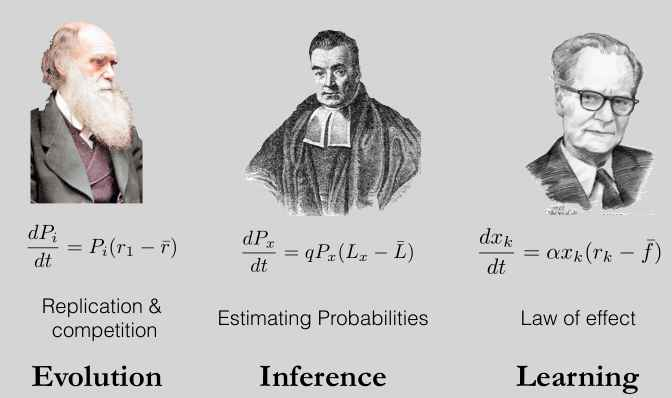
\includegraphics[width=0.8\textwidth]{evolution-inference-learning}
\end{figure}

In other words: a functionalist perspective allows you to see
that the particular mechanical implementation does not matter so much.
All of them achieve the desired goal of maximizing the information in the agent about the world.

\begin{quotation}
	Adaptation is an optimization dynamics transferring information from the environment into the agent--reducing uncertainty about states of the world--\cite{rockmore2018cultural}
\end{quotation}

\subsection{Evolutionary Agents}
So why does an understanding of what an evolutionary agent is help us understand the origin of life, and in particular the multiple origins of life?

It's worth starting with a case study here.
This is Sol Spiegelman; he was a virologist and he was interested in the evolution of very simple viruses.
The virus he worked with was called Q Beta Phage,  a very small RNA virus.
Spiegelman asked the following question: what is the minimum genome the Q Beta has to possess in order to successfully complete its life cycle? But he tricked the virus.
He put a population of viruses in a test tube, along with enzymes that normally it would have to encode itself.
He ensured that those enzymes were always present.
And what he observed, over multiple replication rounds of the virus in its new environment that he created, was that the virus became smaller and smaller and smaller,
until it eliminated all the traces of the enzyme that now existed with certainty in the environment in which it was evolving--Figure \ref{fig:SpiegelmanMonster}. 
\begin{figure}[H]
	\caption{The Spiegelman Monster}\label{fig:SpiegelmanMonster}
	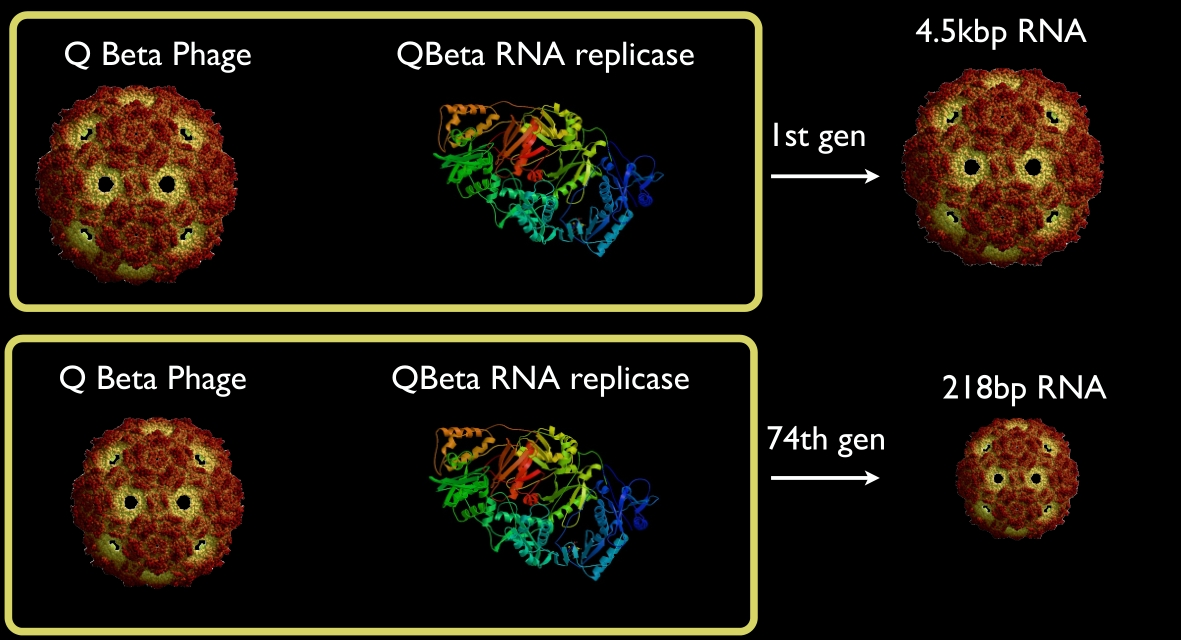
\includegraphics[width=0.9\textwidth]{SpiegelmanMonster}
\end{figure}

We can interpret this experiment in the following way: Figure \ref{fig:SpiegelmanMonsterVenn} depicts a Venn diagram in one set of the viral genome V
and another set, the environment, H, the host.

\begin{figure}[H]
	\caption{Elimination of shared Information}\label{fig:SpiegelmanMonsterVenn}
	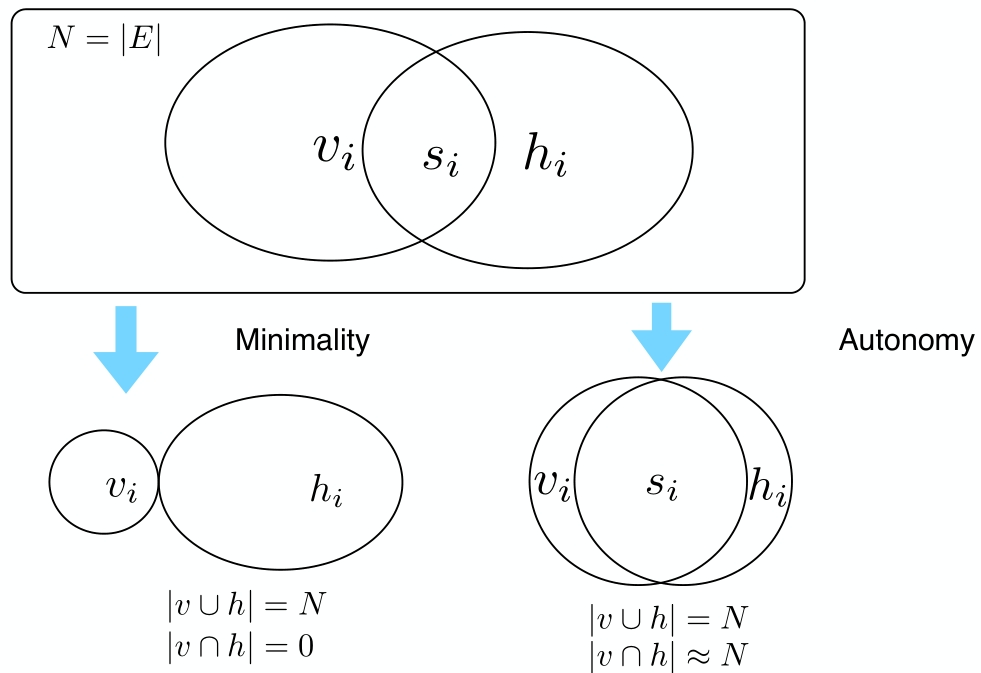
\includegraphics[width=0.9\textwidth]{SpiegelmanMonsterVenn}
\end{figure}
The intersection of these two sets is a gene shared by the virus and the host
or the virus and its environment. 
Spiegelman discovered that if you make the environment certain, the virus minimizes itself.
It throws away all genes it doesn't need because they're already there. This is minimalogy.

But he could have performed an alternative experiment, and made the environment very uncertain.
And when environments are very uncertain, that is, you can't throw things away because you know they'll be there, then you have to encode them intrinsically.

So a good example for us are vitamins.
With respect to vitamins, we're minimal, because we know they're always there and we don't have to synthesize them; but many other genes we can't be certain we can acquire
from the environment, so we have to encode them and transmit them ourselves. And we call that autonomy. So these are two different configurations for an adaptive agent.

Now, many people call a virus "non-living"
because it depends on its host
to replicate, but of course,
we depend on the environment to replicate,
too, because we need vitamins.
So really there is a spectrum of
adaptive agency--Figure \ref{fig:SpectrumOfLife}.

\begin{figure}[H]
	\caption{The Spectrum of Adaptive Agency}\label{fig:SpectrumOfLife}
	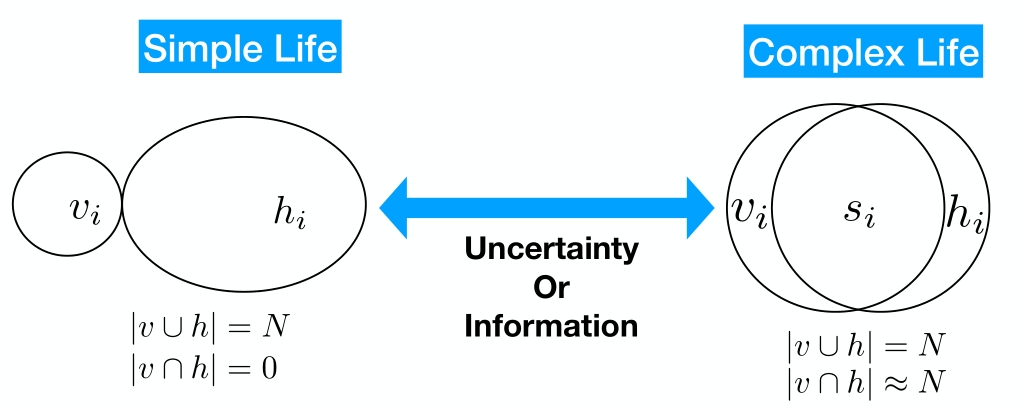
\includegraphics[width=0.9\textwidth]{SpectrumOfLife}
\end{figure}

 On the one hand,
there are organisms that live in very
certain environments. And they become
simple. There are other organisms
that live in very uncertain environments,
and they become complex. They encode
more and more in their genes. And life
spans this informational spectrum, from
organisms that encode very little about
the world because they don't need to,
to organisms that encode a great deal
about the world, because they need to,
to complete their life cycle.

And when you think about it in this
information theory term,
the way an organism, or life,
or an agent really is,
is a mechanism for acquiring adaptive
information about the world that it
propagates forward in time, then
computer viruses, the block chain,
the Constitution, and many many other
cultural forms, are essentially living.

There's nothing special about the biochemical example, a replicated cell, because a replicating cell is simply a somewhat autonomous informational entity that is able to propagate itself forward in time, just like a Constitution can.
But like a virus, the Constitution requires us. We are the vitamins of the Constitution.
And this leads to a very open question that's worth debating.
\begin{itemize}
	\item  On one hand, we could be \emph{fundamentalist}. We could say look, all of life depends on chemistry, and so finding the simplest chemistry that is capable of encoding adaptive information about the world is where life really started.
	\item But another possibility is to say, well not really, because at any scale that you can find this basic set of mechanisms, you're entitled to call it life. And you're even entitled to call it an independent organ of life. So by analogy, someone might say, ''To understand architecture, to understand Gothic and Renaissance, or Baroque, or Rococo architecture, you need understand quantum mechanics''. And I think that would be foolish, because all of them ultimately depend on quantum mechanics, but it's not the differences in the physics that explain the differences in the architecture. That requires a higher level of understanding. And so the \emph{pluralist} approach to the multiple origin of life says that every level, we need to find those unique mechanisms that can support propagation of information. And there isn't a "correct," most basic level. It depends on the question that you're asking and the variation that you're trying to explain.
\end{itemize}

Additional reading\footnote{Personal recommendations by Simon}:
\begin{itemize}
	\item The arrow of time \cite{rovelli2017time,rovelli2019order,susskind2013time}
	\item Information and Life \cite{friston2013life}
\end{itemize}
	
\section[Evolutionary Computation]{Evolutionary Computation--Stephanie Forrest}

Today we're going to talk about how these ideas about evolution look as computations and how we can use computations to understand and leverage 
evolutionary ideas.

Let's first review the three basic elements of Darwinian evolution, which you already learned about.

\begin{itemize}
	\item Random variation of individuals.

	\item Selection of some of those individuals, based on differential fitness
	
	\item Inheritance of those variations into individuals of the next generation.
\end{itemize}

We also need to think a little bit about
how those variations are represented
and that really gets us into the field of genetics
and we don't need to know very
much about genetics, \begin{itemize}
	\item we just need to know that the information, these variations, are represented as discrete units, which today are called genes.

	\item And we need to know that the representation of the information in genes is separate from how it's expressed in the phenotype. So, we refer to this as the genotype versus phenotype mapping.

	\item The final thing we need to know is that these genes are organized in a linear array, which today we call a chromosome.
\end{itemize}

And this understanding really started with Mendel in 1865 and the culmination of it was the Crick and Watson discovery of the structure of DNA.
So, we're going to take those very simple
elements and simple understandings and
translate them into a computer algorithm.
And the way we're going to do that is,
instead of having chromosomes with genes
on them, we're going to have strings with bits--Figure \ref{fig:GeneticAlgorithm}.

\begin{figure}[H]
	\caption[Genetic Algorithm, exhibiting Selection, Crossover, and Mutation]{Genetic Algorithm, exhibiting Selection, Crossover, and Mutation\cite{holland1992adaptation}}\label{fig:GeneticAlgorithm}
	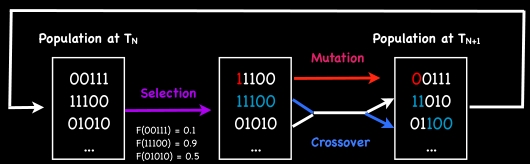
\includegraphics[width=0.9\textwidth]{GeneticAlgorithm}
\end{figure}



Bits are numbers that are either
zero or one, they can only have two values,
and we're going to have those strings of bits
be our individuals in the population.
So, imagine that we start out, and this is
in the left-most panel of the figure.
Imagine that we start out with a population
of randomly generated individuals, or strings,
and here we only have three shown and they
each only have 5 bits, but in real genetic
algorithms we would have more bits and
larger populations.
We also need a way to evaluate fitness
and we do that by using a fitness function.
In our example fitness function, we will assume
that the values range from 0 to 1 and the
higher value (1) is better.

So, the first step is generate initial population,
then we need to evaluate each individual
in the population using our fitness function
and use those fitness values to select
the next generation.

And so, you see that in the center panel
where we have two copies of the highest
fitness individual, no copies of the lowest
fitness individual, and a single copy
of the average individual.
That's not very interesting because
those individuals look exactly like their parents.
And so, we take advantage of what are known as
genetic operators to introduce new variations.
And we do that using mutation that's shown
in the top individual where the first bit (a one)
is flipped to become a zero, and we do this
not always in the first position, we do it
randomly at different places in the string,
and do it randomly throughout the strings
of the population.

Then we also use a process called:
crossover, or recombination, where we take
two individuals and exchange pieces of their
DNA or pieces of their bit strings, and
you see that in the second two individuals.

So, now in the third panel, we have the

true, new generation, Generation T+1, and
we then need to repeat the cycle
and evaluate those using the fitness function,
do new selection, introduce new mutations
and crossovers, and that is how
the evolutionary process runs.
This basic strategy, and basic idea of using
bit strings to represent chromosomes was
introduced by John Holland in the early 1960s.
John was very interested in the
populations level effects and in the
impact of crossover.

Coming back to the algorithm,
what does it look like when we actually
run this algorithm for multiple generations?
So, I just showed you one generation in the previous slide,
but we typically iterate these for hundreds
or even thousands sometimes, of generations.
And the way we look at it is by plotting time
in terms of numbers of generations on the x-axis
and the fitness, typically the average fitness
of the population or the best fitness of
the population. Those are the two values
shown  on the y-axis-- Figure \ref{fig:GAfitness}.

\begin{figure}[H]
	\caption{Example Fitness Curve, with two plateaux}\label{fig:GAfitness}
	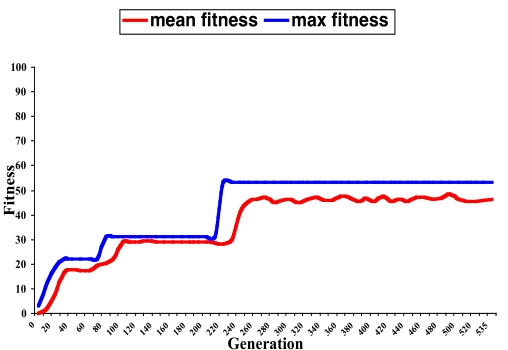
\includegraphics[width=0.9\textwidth]{GAfitness}
\end{figure}
And so, this is a very typical kind of
performance curve that we see with genetic
algorithms, where the fitness of the population
starts out very low initially, very quickly
climbs up and improves as the really lousy
individuals get deleted and the somewhat
better individuals get copied, so the whole
average fitness moves up.
Then there's a little bit of searching around
that we see, and we get another innovation.
But eventually, the population gets stuck
on what is known as a plateau.
This is known as punctuated equilibrium.
And when that happens, then the algorithm
is affectively having to explore the space
more widely to find a high fitness
innovation and so that can take a varying
amount of time, and we actually see two
plateaus, the first plateau we see in the figure
we see eventually and new innovation is found
and the population jumps up in fitness
and this is very typical of these
genetic algorithms.

Let's now talk about some applications.
Genetic algorithms have been used widely
in engineering applications and they've
also been used for scientific modeling.
First, we'll talk about the engineering
applications, and of these by far the
most common is what's known as
multi-parameter function optimization--Figure \ref{fig:multi-parameter-optimization}.

\begin{figure}[H]
	\caption[Multi Parameter Optimization]{Multi Parameter Optimization\cite{marshall2014evolution}}\label{fig:multi-parameter-optimization}
	\begin{subfigure}[h]{0.5\textwidth}
	\caption{2D fitness surface\cite{marshall2014evolution}}\label{fig:multi-parameter-optimization-2d}
		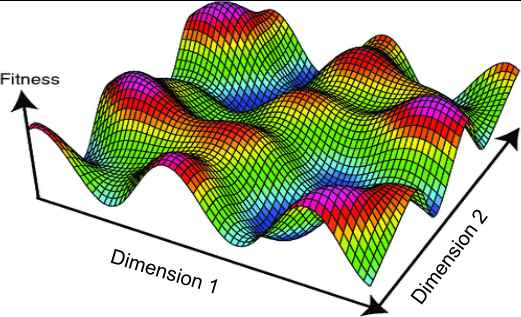
\includegraphics[width=\textwidth]{multi-parameter-optimization}
	\end{subfigure}
	\begin{subfigure}[h]{0.45\textwidth}
		\caption{Example function}\label{fig:multi-parameter-optimization-example}
		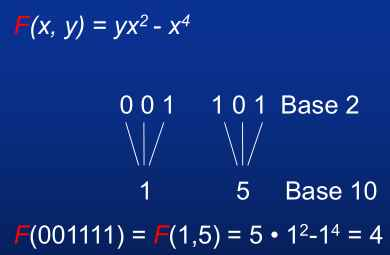
\includegraphics[width=\textwidth]{multi-parameter-optimization-example}
	\end{subfigure}
\end{figure}

Figure \ref{fig:multi-parameter-optimization-2d} depicts
a two-dimensional function,
that is a function in two variables.
And if a function is complex a lot of times
we don't have analyticity methods to find mathematically
what the maximum value of the function is
and when that happens we have to resort to
sampling and we can think of the genetic algorithm
as a kind of biased sampling algorithm.
And the goal, of course, would be to find
in this multi-peaked surface points that
are on the highest peak up at the top.
Let's just go into a little bit more detail
about how that works.
Figure \ref{fig:multi-parameter-optimization-example} depicts an example of such a function and it's not trivial to analyze this mathematically,
but suppose we want to find the x and y values
for this function that produces the
maximum F(x,y).

So to do that, we take out bit strings and
conceptually think of the first half of the
string as being a representation of the
value of x, and the second half of the string
is being a representation of the value of y.
Now, to evaluate fitness we then need to
take these ones and zeros and interpret
them as Base 2 numbers, translating them
into their decimal equivalents, which is
shown on the figure, and then take those
decimal values and plug them into our
fitness function, and in this case we get
the value out 4.

So, we would have to do that for every
individual in the population.
I just want to say a word about where
these algorithms came from. I've mentioned
John Holland. There were several other
groups that were interested in similar
kinds of algorithms and the first three main
groups I've listed were all independent
discoveries of similar and overlapping ideas.
And then in the early 90s, John Koza\cite{koza1992genetic} came along
and really blew open the field by showing
how we could use genetic algorithms to
evolve computer programs.
These separate stream inventions are now
lumped together and the field is called
Evolutionary Computation.

And needless to say, there's been
a lot of recombination between these
different origins.


References

\begin{itemize}
	\item John Holland \cite{holland1992adaptation}
	\item Ingo Rechenberg \cite{rechenberg1965cybernetic}
	\item David Fogel et al\cite{fogel1998artificial}
	\item John Koza--evolving computer programs\cite{koza1992genetic}
\end{itemize}

See also \cite{mitchell1998introduction,eiben2003introduction,forrest1993genetic,ma2014novo}.

\section[Scaling]{Scaling--Pablo Marquet}

Why is scaling important and why do you need to know about this?
\begin{itemize}
	\item Scaling provides a way to deal with the diversity of scales and also the... different type of organism that exists and becomes part of ecological systems.
	\item Scaling also makes apparent the fundamental similarity that underlies the diversity in nature and how this has been moulded by the action of natural selection. It's very important to realize that scalings point out that there are not many ways of actually having a real functioning organism in nature and provides you with the right way of understanding the constraints that are operating on diversity. And, since most organisms obey these constraints, it points to the fundamental similarity that they share.

	\item Scaling provides us with a  benchmark against which we can compare different species, populations and ecosystems, and you can actually measure deviations from scaling relationships, and those deviations mean that there are some processes--some important biological processes--operating on these systems
\end{itemize}.

So, let's start by the most simple way of characterizing scaling in ecology.
And, the characterization is a mathematical one - it's very simple.
And usually, scaling relationships, as you have already heard, cannot be summarized with
a relationship like a variable $y$ or a trait of an organism.
It is proportional to a variable $M$ raised to a power.
In this case, I'm talking about $M$ as the mass of the organism or the size of the biological system. You can also represent this relationship as $y=c M^\alpha$ which actually allows you to take the logarithm of this relationship and transform something which is not linear into a linear equation--(\ref{eq:PowerLawScaling}) and Figure \ref{fig:PowerLawScaling} .
\begin{align*}
	y \propto& M^{\alpha}\text{, where $M$ represents mass, size, etc.}\numberthis\label{eq:PowerLawScaling}\\
	=& c M^{\alpha}\\
	\implies&\\
	\log(y)=&\log(c) + \alpha \log(M)
\end{align*}

\begin{figure}[H]
	\caption[Many ecological attributes scale with size]{Many ecological attributes scale with size\cite{white2012methodological}}\label{fig:PowerLawScaling}
	\includegraphics[width=0.9\textwidth]{PowerLawScaling}
\end{figure}

On the left you see scaling relationships that are in the nonlinearized way. And then, to the right you see the linear relationship that results after you take the logarithms
of this relationship.
That makes it easier to analyze.
So, examples of scaling abound in nature
and they affect the way organisms
are put together and evolved
through the action of natural selection.
You can see, for example,
relationships between
the size of the organisms
and weaning time,
or also, the size of the organisms
and longevity.

And, you can use this relationship -
as I show you here in Figure \ref{fig:ScalingExamples} -
to compare different kinds of organisms.
\begin{figure}[H]
	\caption[Scaling of life-history events]{Scaling of life-history events: mammals are in grey, marsupials in red.\cite{sibly2012metabolic}}\label{fig:ScalingExamples}
	\includegraphics[width=0.9\textwidth]{ScalingExamples}
\end{figure}
For example, the gray dots represent
all mammalian species
and the red dots represent
one particular type of species,
which are the marsupials.
So, you can see the marsupials, they...
in general, they follow the trend's line
for longevity, for example,
but they deviate in maturation time,
for example.
So, these scaling relationships
allow you to compare
and you can use them as a benchmark
to try to understand what is going on
with this particular species
that they deviate.
Is this because of
their phylogenetic history?
Or, is it because of the environment
of the other kind of habits they have -
what they eat and so on.
So, you can answer
meaningful questions
using the scaling relationships.

In ecology,
these relationships also affect,
for example, things very fundamental,
like the average prey mass
that a particular carnivore species
will eventually eat,
or affect, as you can see in Figure \ref{fig:Scaling:individuals:ecosystems},
the carbon turnover,
or the time it takes,
to replace one gram of carbon
in a particular ecosystem
and how that changes
with the average mass of the plants
in that ecosystem.

\begin{figure}[H]
	\caption{Scaling in individuals and	ecosystems}\label{fig:Scaling:individuals:ecosystems}
	\begin{subfigure}[b]{0.45\textwidth}
		\caption{Mean Carnivore Mass\cite{tucker2014evolutionary}}\label{fig:mcm}
		\includegraphics[width=\textwidth]{Scaling1}
	\end{subfigure}
	\begin{subfigure}[b]{0.45\textwidth}
		\caption{Carbon Turnover\cite{anderson2013altered}}\label{fig:ct}
		\includegraphics[width=\textwidth]{Scaling2}
	\end{subfigure}
	\begin{subfigure}[b]{0.45\textwidth}
		\caption{Primary Production\cite{enquist2012land}}\label{fig:npp}
		\includegraphics[width=\textwidth]{Scaling3}
	\end{subfigure}
\end{figure}

Or also, you can see scaling
relationship in terms of
the net primary productivity
of an ecosystem
and the total amount of
plant biomass in that ecosystem.
So, those are fundamental relationships
that tell you something very... general
about the way organisms
and ecosystem work.

So how do we understand
the origin of this relationship?
Well, let me tell you, the fundamental...
kind of relationship I would say is
the one that relates the organism
and its energy requirement to its size--Figure \ref{fig:Kleiber}.

\begin{figure}[H]
	\caption[Kleiber's Law]{Kleiber's Law: $B \propto M^\frac{3}{4}$\cite{schmidt1984scaling}}\label{fig:Kleiber}
	\includegraphics[width=0.9\textwidth]{Kleiber}
\end{figure}

This is called "Kleiber's Law,"
and it points out that
the requirements of energy
of an organism, its metabolism,
which is the sum of
all the biochemical reactions
happening within the organism,
scale with the size of the system -
or mass -
raised to a three-quarters power.
And, you can see in the graph that
this relationship describes very well
how metabolism changes
as you increase the mass of an organism
from a mouse, for example,
to an elephant.
And, it tells you that somehow
an elephant is just a variation
on the same theme as a mouse is.
So, it's this relationship that points out
that there is a fundamental similarity
among these different kinds of organisms.
So, natural selection
is not acting randomly -
it's following some constraints or...
so, what are those constraints?

In 1997, Geoffrey West, Jim Brown and Brian Enquist, proposed a very simple and elegant model that points out to some fundamental principles acting and helping us to understand why metabolism changes in the way it does with the size of a system.
And, I'm not going to explain to you
all the details of the model.
I'm just going to give you
two major insights into it.
\begin{itemize}
	\item The properties of resource delivery networks determine
	the properties of whole-organism metabolic rate.
	\item  Biological systems have evolved under natural
	selection to optimize performance (delivery networks
	minimize energy loss)
\end{itemize}

Well, the major thing is that
any organism that exists faces a problem
and the problem is that
you have to deliver energy -
the resources that you get
from the environment to live -
you have to deliver it to
all the different parts of your body.
In a multicellular organism,
this means that you have to deliver
this energy to all the cells in your body--Figure\ref{fig:capillaries}.
\begin{figure}[H]
	\caption[The West, Brown, Enquist Model]{The West, Brown, Enquist Model; In a multicellular organism, you have to deliver energy to all the cells in your body.\cite{west1997general}}\label{fig:capillaries}
	\includegraphics[width=0.8\textwidth]{capillaries}
\end{figure}
So, how do you do that?
Well, the way you do that is
you construct.
I mean natural selection has molded
the existence of networks
to deliver this energy towards
all the parts of your body.
So, those networks
actually generate constraints
that manifest in this fundamental
three-quarter scaling for metabolism.

Now, the way natural selection
acts on this is
by minimizing energy loss.
So, it generates networks
that minimize this energy -
so efficient networks -
when you take account of what
you consider these two major insights,
and they show
in a mathematical model
that this creates the three-quarter
scaling relationship that we see.
So, let me give you some example
of the implications of this relationship
in ecology.

One simple one is that you can ask
a very simple question like -
what is the maximum number
of individuals
that can be found in a given area?
So, to answer this question,
which I think is a very fundamental one,
you are just required to know
the amount of energy or resources
that are in a particular area,
and the requirements of those resources
by different kinds of individuals.
So... we know that the scale
with the size of the organisms
rises through three-quarters.
So, it's very simple then to compute
the maximum number of individuals
in a given area
just by dividing the amount of resources
over the requirements of each individual.
What that gives you is
another scaling relationship
that says that the maximum number
of individual scales with mass
raised to minus three quarters.

\begin{align*}
	R=& \text{Energy or resources per unit area}\\
	B=&\text{Individual resource requirements}\\
	N_{max}\propto& R M^{-\frac{3}{4}}\label{eq:max}\numberthis
\end{align*}

Now, let's see the empirical evidence.
The empirical evidence on this,
and I'm going to go back
to a paper published by
John Damuth in 1981
where he made a compilation
of the density
of different mammal species
around the world.
And, these happened to be
every [major] mammal...
and he computed the density
and size of each of these species,
and he plotted this relationship,
and, as you can see in  Figure \ref{fig:MammalianHerbivores},
there's a negative slope and
this slope is minus three quarters.

\begin{figure}[H]
	\caption[Mammalian Herbivores]{Mammalian Herbivores--$N_{max}\propto R M^{-\frac{3}{4}}$\cite{damuth1981population}}\label{fig:MammalianHerbivores}
	\includegraphics[width=0.9\textwidth]{MammalianHerbivores}
\end{figure}	

So, right as predicted,
the maximum number of individuals
follow a minus three-quarter
scaling law.
The implications of this
are very interesting
because it means that mice actually...
they achieved larger densities
than elephants,
but somehow they are the same,
because they, as I will show you,
they use the same amount of energy
at the population level.
And, how we can calculate that?
Well, we call that
the "population energy use."
Population energy use - PEU -
is proportionate to
the number of individuals times
the requirements for energy.
So, that will be the total amount
of energy required by a population.

And, if we replace the known
scaling relationships
for number and for energy requirements,
we know that population energy use
will be proportional to
mass raised to minus three quarters
times mass raised to three quarters.
As you can see from (\ref{eq:const}), these two exponents
they kind of annihilate themselves
and give you a population energy use
that is proportional to
mass raised to zero,
meaning that population energy use
tends to be invariant
regarding the size of the organisms,
meaning that elephants use
the same amount of energy
that mice use--Figure \ref{fig:PopulationEnergyUse}.
\begin{align*}
	E_{pop}\propto&N B\text{, Energy use for population}\\
	\propto& M^{-\frac{3}{4}} M^{\frac{3}{4}}\\
	\propto& 1\label{eq:const}\numberthis
\end{align*}
\begin{figure}[H]
	\caption[Population Energy Use]{Population Energy Use\cite{enquist1998allometric} }\label{fig:PopulationEnergyUse}
	\includegraphics[width=0.9\textwidth]{PopulationEnergyUse}
\end{figure}

So, this is a very fundamental
invariant relationship.
There are many more scaling relationships
that show this kind of property
of invariance,
but it shows you that
things can be different,
but at the same,
time things can be equal
if you explore this relationship
between the scalings.

So, why is it fundamental?
Why is this very important too
is because it allows us to understand
something about ourselves too.
And here, I want to make the point that,
using this relationship,
you can understand that humans
are a hyper-dense species--Figure \ref{fig:Hyperdense}.
\begin{figure}[H]
	\caption{Humans--the hyper-dense species}\label{fig:Hyperdense}
	\includegraphics[width=0.9\textwidth]{Hyperdense}
\end{figure}
How do we know that?
Because, we know the scaling
relationship for all mammals.
We know how density changes as you
change the body size of the mammal.
We are mammals.
On average, a human being
you can consider weighs around 70 kilos.
And, you can try to plot which would be
the density that we should achieve
if we will kind of
follow this relationship.
And, our density will be around
2.12 individuals per square kilometer.
So, the realized density is
5.8 raised to 10 to 4 [fourth power]
meaning 58,000 times larger.

So, this is a very significant deviation
from the expected scaling relationship.
And, this is a very meaningful one
because
you can now answer how it comes -
what happens to humans
that they could shift to
such an extreme maximum density
as it does these days.
Well, let me tell you that
when we were in a different kind of
stage of development,
a social stage of development -
when we were hunter-gatherer -
we really fit into this relationship.
As we moved through time
and social complexity,
we were moving away
from this relationship
and now we are far away from it.
And, this has impacts in terms of
the amount of energy that we use
and the impact of that amount of energy
used by humans
on the rest of the ecosystem.
That is called, or is part of
what we call "global change."

We're not going to deal with this
in this class,
but it's important to keep it in mind.
That's why scaling relationships help you
to realize there are similarities,
there are fundamental principles
related to the way
organisms deliver energy
through networks
that explain the amount of energy
that different organisms require
and this constrains the density
and amount of energy
their populations use.
And... you can use them
to understand deviations,
like the humans' density extreme
or hyper-density of humans now.

See also \cite{white2012methodological,sibly2012metabolic,tucker2014evolutionary,anderson2013altered,enquist2012land,west1997general,damuth1981population,enquist1998allometric,marquet2005scaling} 

\section[Energy]{Energy--Van Savage}


Today I'm going to talk to you
about energy in biology.
"In biology" I mean all of biology,
from evolution to ecology,
to physiology to cellular biology.
And, the reason I can talk to you about it
from such a wide swathe of biology
is because we use energy
for everything we do
and because we spend a lot
of our time and abilities
just trying to get energy
and make energy.
For those reasons,
there's infinitely many ways
in which I could talk about energy
and infinitely many ways
I could describe it to you,
but one of the most fun things to me
and one of the arts of science to me
is deciding how to draw the boxes
that we're gonna use.

And, to do that,
you often have to frame a question
or think about some objective
you're trying to meet.
And, the two I'm going to talk about
in this talk:
\begin{enumerate}
	\item one is with relation to evolution--how do we think about energy in terms of evolution and what's needed for evolution?

	\item And, the other is more in relation to physiology and ecology, which really has to do with how do we get energy and how do we make energy.

\end{enumerate}

So, from an evolutionary perspective,
the main thing we are concerned about
is fitness,
which is how many offspring
or individuals
we give to the next generation.
To do that, we first have to grow
and maintain ourselves to reproduce.
So, one of the main boxes for evolution
actually is development and growth.
So, Figure \ref{fig:development} shows a plant growing
from early stages to later,
and, in doing that,
it has to create many more cells,
it has to create new types of cells
and new types of structures -
so this takes a lot of energy
and is a very energy intensive process.

\begin{figure}[H]
	\begin{center}
		\caption{Plant growing
			from early stages to later}\label{fig:development}
		\includegraphics[width=0.6\textwidth]{development}
	\end{center}
\end{figure}
And, that's also true
for animals and their growth.
Figure \ref{fig:animals} is a picture of these two birds
crying out to their parents for food -
to bring them food -
because they need lots more food
to grow and have energy
to get to be big enough to reproduce.
\begin{figure}[H]
	\begin{center}
		\caption{Two birds
			crying out to their parents for food}\label{fig:animals}
		\includegraphics[width=0.6\textwidth]{animals}
	\end{center}
\end{figure}

The next box I'll talk to you about
for energy is maintenance,
and that's sort of a less obvious
visible one
because you're not seeing cells change
or structures change or reproducing -
you sort of see things
staying the same way they are visibly,
but actually that takes a lot of energy
just to replace cells that die
or to feed cells energy
just to keep living.
As extreme examples,
if you look at the redwood trees--Figure \ref{fig:maintenance}--
it takes an enormous amount of energy
just to keep water or sap
pumping up to the leaves at the top -
it's a huge distance they have to travel.
\begin{figure}[H]
	\begin{center}
		\caption{Redwood trees}\label{fig:maintenance}
		\includegraphics[width=0.6\textwidth]{maintenance}
	\end{center}
\end{figure}
And, you have to build structures
to maintain them to go up to these leaves.
So, you use a lot of energy
just to keep pushing
up to the tops of the trees.
And, similarly, we use energy
for all the structures in our body.

But, there are extreme examples here too
where -
if we're thinking about a peacock--Figure \ref{fig:peacock}
if it builds a whole array of feathers,
that takes a lot of energy to build
and to maintain.

\begin{figure}[H]
	\begin{center}
		\caption{It takes a lot of energy to build a peacock's feathers.}\label{fig:peacock}
		\includegraphics[width=0.6\textwidth]{peacock}
	\end{center}
\end{figure}

And, it's going to use that
to attract a mate,
which it again
it needs for reproduction,
which is important for evolution.

As a brief aside,
before I get to reproduction,
from maintenance,
one of the interesting things to me
about us as humans is that,
individually biologically,
we use about the same amount of power
or energy per time
that you would see in a light bulb,
but once you add in things -
how much energy we use for cars
or computers or light bulbs
or heating our houses -
we actually, each individual in the US,
uses about the same amount of energy
as a blue whale,
so we're really enormous energy users
in terms of our biological footprint.

The last evolutionary box I'll talk about
for energy is reproduction,
which is where evolution sort of
ultimately aimed most of the time.
And, that can be things
like oranges on a tree
that tempt us to eat them
because they're so pretty
and flavorful and taste good,
and then, we walk around
and distribute those seeds
to help our orange trees grow elsewhere
and increase their numbers.

Or also, an embryo
growing inside a mother
that takes a huge amount of energy
and time to produce
that's necessary for reproduction.

So, growth, maintenance
and reproduction
are the main boxes that I think
you can think about for evolution
where energy is needed.
But now, I'm gonna shift gears
and talk a little bit more
about how it's needed
for physiology and ecology,
which has a lot to do with
how do you get energy
and how do you make energy,
which evolution still plays a big role in
because you need those things to survive,
but it's not as explicit as
if you do it this way.

So, in terms of obtaining energy,
Figure \ref{fig:owl-mouse} is a dramatic picture of an owl
chasing down a mouse to eat for food,
and that's one type of example
of getting resources or food
through what we call "active capture."
But, other ways include things
like grazing - like a cow in a pasture,
or "sit-and-wait,"
which would be like snakes or spiders
waiting for prey items to come to them.

\begin{figure}[H]
	\caption{How to obtain energy}
	\begin{subfigure}[t]{0.3\textwidth}
		\caption{Owl chasing mouse}\label{fig:owl-mouse}
		\includegraphics[width=\textwidth]{owl-mouse}
	\end{subfigure}
	\;\;\;
	\begin{subfigure}[t]{0.3\textwidth}
		\caption{Owl chasing mouse}\label{fig:tree-above-ground}
		\includegraphics[width=\textwidth]{tree-above-ground}
	\end{subfigure}
	\;\;\;
	\begin{subfigure}[t]{0.3\textwidth}
		\caption{Owl chasing mouse}\label{fig:tree-roots}
		\includegraphics[width=\textwidth]{tree-roots}
	\end{subfigure}
\end{figure}

And also, plants are a little bit
like that
in terms of getting energy.
They're more like sit-and-waits,
where they build structures
and wait for things to come to them.
So, as we see in Figure\ref{fig:tree-above-ground}, there's an extensive
branching system for this tree,
and when the leaves are all present
on the limbs,
it's using that to get light from the environment,
and get as much light in this little area
as it can - within that canopy.

And, that sort of branching system
is reflected below ground
in terms of root systems
that it uses to get water nutrients
from the ground as well,
where it has to branch out
and get as much resources as it can--Figure \ref{fig:tree-roots}.

Once resources are obtained,
we have to process that to make energy,
and, the first step in that for animals
is the digestive system,
which, you know, involves 
going through our stomachs
and things like that.
But, the part I want to highlight here--Figure \ref{fig:digestion}
is that, in our guts,
there are these microbial systems,
often now called the "microbiome"
or the "gut microbiome,"
which we have to have
to process energy.

\begin{figure}[H]
	\begin{center}
		\caption[The gut microbiome]{In our guts, there are these microbial systems, often now called the "microbiome" or the "gut microbiome," which we have to have to process energy}\label{fig:digestion}
		\includegraphics[width=0.6\textwidth]{digestion}
	\end{center}
\end{figure}

It's this own little world -
an ecosystem - inside our bodies.
And, basically, based on how it processes
energy and the energy it needs,
it really affects which bacteria you see
and the diversity of bacteria you see,
and when that's off
it can really affect our digestive system.

After we process energy
and get it in a more usable form
from what we took into our bodies,
we still have to get it
to the rest of our bodies -
to our fingertip, our toe tip,
or our head to use,
and that's done by a branching system
inside our bodies--Figure \ref{fig:distribution1}.
It looks a lot like the branching system
in trees outside
or in their roots in the ground -
and that's the cardiovascular system,
where we use a heart to pump blood
out to our limbs and to our head.
And then, at the finer scale,
we have capillaries or capillary beds--Figure \ref{fig:distribution1},
which is where the transfer of oxygen
or other nutrients can take place.
\begin{figure}[H]
	\caption{Distributing Energy}
	\begin{subfigure}[t]{0.4\textwidth}
		\caption{The cardiovascular system}\label{fig:distribution1}
		\includegraphics[width=\textwidth]{distribution1}
	\end{subfigure}
	\;\;\;
	\begin{subfigure}[t]{0.55\textwidth}
		\caption{Capillaries}\label{fig:distribution2}
		\includegraphics[width=\textwidth]{distribution2}
	\end{subfigure}
\end{figure}


Once we distribute energy
and get it to each cell that needs it
to keep producing energy and living,
the main way we make energy -
at least in animals -
is through mitochondria,
and each mitochondria
is like a little engine
that takes oxygen and makes energy.
And, it's actually a really old bacteria
that we've brought in to -
not "we" humans -
but a long time ago
cells brought in to make energy for them.
So, it's a really ancient way
of making energy.

That leads to the question:
if it's really ancient,
is it really good at it -
is it very efficient?
And, I would think it would be
because, if it's used that broadly,
you would think it must be pretty good
or you would reinvent the wheel somehow.
But, what's interesting is
if you compare to something like solar panels,
and compare like the grass
and the trees in the background here
to the solar panels in the foreground,
the grass and the trees
use photosynthesis to make energy,
which is about three percent effective,
but the solar panels can get up to
about 30 percent efficiency,
so about 10 times better,
which was kind of shocking to me
when I first learned about it -
that they can do so much better.
And, maybe this does suggest
that biology can still evolve
and do better.

But, the catch here really is that
solar panels use a lot of elements
that aren't easily accessible
to biological organisms -
they take money to to either mine
or to construct them the right way.
When we think about
sort of being efficient or evolving,
it's always within constraints.
So, I'd argue that biology is applied
really well in the constraints it has,
but we're able to get at things
biology has not been able to get to.

And, looking at this efficiency question
from a different perspective,
if you think back again to the networks,
either for trees or the cardiovascular
system within our bodies,
there's a million ways
you could build such a network.
We want those networks to span space
to be able to get blood or water
everywhere it needs to go,
and we want them to do so
in an efficient way
so we don't spend
a huge amount of energy
just pumping blood around
and losing energy pushing fluid around.
And, if you think about all the ways
in which networks could be built,
you can look at... drive theory
and look at data
to see what's the most optimal.
And, it turns out that biology
has done a really good job
of optimizing networks to be efficient

And, one consequence of that,
actually, as you look at metabolic rates
on the y-axis in Figure \ref {fig:MammalianBasalMetabolicRate}
versus mass on the x-axis,
you see a very clean systematic pattern
where, the bigger something is,
the more energy it uses -
which isn't surprising.

\begin{figure}[H]
	\caption[Metabolic rate depends on optimized networks and body size]{Metabolic rate depends on optimized networks and body size\cite{savage2004predominance}}
	\begin{subfigure}[p]{0.45\textwidth}
		\caption{Mammalian Basal Metabolic Rate}\label{fig:MammalianBasalMetabolicRate}
		\includegraphics[width=0.9\textwidth]{MammalianBasalMetabolicRate}
	\end{subfigure}
	\begin{subfigure}[p]{0.45\textwidth}
		\caption{Whole Plant Xylum Flux}\label{fig:WholePlantXylumFlux}
		\includegraphics[width=0.9\textwidth]{WholePlantXylumFlux}
	\end{subfigure}
\end{figure}


But, the surprising piece here
is that it's nonlinear.
So, you think about an elephant
that's 10,000 times bigger than a mouse,
it only uses about
a thousand times more energy,
which means - per cell -
a cell from an elephant
uses about ten times less energy
than a cell from a mouse.
So, you're gaining efficiency
by getting bigger
in this way of looking at it.
And, just to make sure for people
paying close attention to the axes here,
they're logarithmic axes -
so a curved line becomes a straight line,
and, what would be the exponent
of a mathematical equation
becomes the slope.
And, this pattern is true,
not just for across these large...
huge range of sizes
in mammals or animals in general,
but also for plants -
xylem flux is a similar sort of measure
of metabolic rate in plants.
We plot that versus body size again--Figure \ref{fig:WholePlantXylumFlux}--
and again, you see
a very clear straight line
across a huge range in size for plants,
and, again,
an exponent or a slope
that's close to 3/4.
So, the same sort of pattern
shows up again.

And, another big effector,
besides body size--after body size,
the biggest effector of energy use
across individuals is temperature.
So, if you look in --Figure \ref{fig:BodyTemperature},
basically the warmer something is--
if we think about a frog
or a turtle or a plant--
the warmer it is,
the faster it uses energy,
and that increases at exponential rates
that are faster and faster and faster
up to the point where
you get extreme temperatures
and things start to fall apart
and things just start to die.

\begin{figure}[H]
	\caption[Metabolic rate depends on body temperature]{Metabolic rate depends on body temperature\cite{dell2011systematic}}\label{fig:BodyTemperature}
	\includegraphics[width=0.9\textwidth]{BodyTemperature}
\end{figure}

But, up until that point or close to it,
the warmer you are
the faster you use that energy.
And because, as we started seeing
at the start of this talk,
that we use energy for everything we do,
understanding how mass
and temperature affect metabolic rate
or the power we produce
tells us a lot about all kinds of
other things in biology.

So, for example, if we look at
heart rates across mammals--Figure \ref{fig:MammalianRestingHeartRate},
another way to think about this
in terms of mouse versus elephant
is that an elephant's heart beats
about ten times slower than a mouse.
So, every time an elephant's heart
beats once,
the mouse will have beat
ten times really quickly.


\begin{figure}[H]
	\caption[Mammalian Resting Heart Rate]{Mammalian Resting Heart Rate\cite{savage2004predominance}}\label{fig:MammalianRestingHeartRate}
	\includegraphics[width=0.9\textwidth]{MammalianRestingHeartRate}
\end{figure}


Or, if you look at ecology--Figure \ref{fig:AndEcology}--
when we correct for temperature
and like versus size
and we think about how much
each individual produces in a system,
that actually follows a very tight,
clean pattern here as well
and it's true across a huge,
diverse variety of taxa
that includes plants, mammals,
insects, fish -
almost everything you can think of.

\begin{figure}[H]
	\caption{Ecology and Temperature Correction}
	\begin{subfigure}[b]{0.5\textwidth}
		\caption{Temperature Corrected Individual Production\cite{ernest2003thermodynamic}}\label{fig:AndEcology}
		\includegraphics[width=\textwidth]{AndEcology1}
	\end{subfigure}
	\begin{subfigure}[b]{0.5\textwidth}
		\caption{Temperature Corrected Population Density\cite{ernest2003thermodynamic}}\label{fig:AndEcology2}
		\includegraphics[width=\textwidth]{AndEcology2}
	\end{subfigure}
\end{figure}

And finally, as another ecological example--Figure \ref{fig:AndEcology2}--
this affects how many individuals per area
that we see; the bigger you are
or the warmer you are,
the more energy you need
the fewer individuals you get around.
And, you see this systematic pattern
for animals,
which are the red dots
and plants,
which are the green dots.

And, one of the interesting things here
is that animals are much lower
than the plants
and that's because it has
conversion efficiency,
where plants have to convert
sunlight into energy,
and, basically, all animals
either directly or indirectly
get their energy from plants.
So, they get about ten percent
of the energy from plants
that they can use
to produce their numbers.
So they're lower down
because they lose a lot of efficiency
in going from plants to animals.

References: \cite{sibly2012metabolic,battley1987energetics,odum1976energy,odum1983systems,schmidt1997animal,brown2004toward,kempes2017thermodynamic}.

\section[Nonequilibrium Physics]{Nonequilibrium Physics-- Eric Smith}

We will talk about how motion itself can freeze. Topics covered:
\begin{itemize}
	\item The equilibrium concept of phase transition
	
	\item How phase transitions explain robust patterns
	
	\item Why equilibrium isn’t enough to understand life
	
	\item Phase transitions in dynamical systems--''frozen motion''
\end{itemize}

\subsection{Phase Transitions}

To understand what makes phase transitions special we have to start with the ''ordinary'' response of thermodynamic systems to controls. E.g. lava has viscosity, which increases smoothly as temperature is lowered--Figure \ref{fig:lava}.

\begin{figure}[H]
	\begin{center}
		\caption[The ''ordinary'' response of thermodynamic systems to controls]{The ''ordinary'' response of thermodynamic systems to controls.  Hot lava flows like water: viscosity increases smoothly (gradually!) as temperature is lowered.}\label{fig:lava}
		\includegraphics[width=0.8\textwidth]{lava}
	\end{center}
\end{figure}


 Phase transitions are different:
\begin{enumerate}
	\item Water does not become harder as it is cooled
	\item It turns to ice suddenly at a ''critical temperature''--Figure \ref{fig:water-ice}.

	\begin{figure}[H]
		\begin{center}
			\caption{Phase transitions are different}\label{fig:water-ice}
			\includegraphics[width=0.8\textwidth]{water-ice}
		\end{center}
	\end{figure}

	\item The average direction of pointing of the ice sharply increases from zero at the freezing temperature--Figure \ref{fig:water-ice1}.
	\begin{figure}[H]
		\begin{center}
			\caption[The suddenness of change matters]{The suddenness of change matters. At the left the water models point in no particular direction.}\label{fig:water-ice1}
			\includegraphics[width=0.8\textwidth]{phase-transition1}
		\end{center}
	\end{figure}
	\item The direction and strength of the crystal is called the ''Order Parameter'' of the transition--Figure \ref{fig:water-ice2}. They give a sense of what kind, and how much order it has. The order parameter's direction is arbitrary, and the strength has to do with how far we are below the freezing temperature. It gives an idea of how globally the ice crystals are lined up, and how rigidly.
	\begin{figure}[H]
		\begin{center}
			\caption{Concept of an order parameter}\label{fig:water-ice2}
			\includegraphics[width=0.8\textwidth]{water-ice2}
		\end{center}
	\end{figure}


	\item Change is sudden because ''you can’t have half a symmetry''--Figure \ref{fig:water-ice3}.
	\begin{figure}[H]
		\begin{center}
			\caption{You can’t have half a symmetry}\label{fig:water-ice3}
			\includegraphics[width=0.8\textwidth]{water-ice3}
		\end{center}
	\end{figure}
	\begin{itemize}
		\item A direction either exists or it doesn’t
		\item The water is symmetric, so all frozen directions are equivalent. In order the freeze you must choose one. It is the choice that gives rise to the suddenness with which the transition sets in. This causes phase transitions to play a very important role in our material world. They are responsible for most of the robust patterns that we see.
	\end{itemize}
	\item Phase transitions, cooperatively-maintained states, and robustness--Figure \ref{fig:a-girls-best-friend}.
	\begin{figure}[H]
		\begin{center}
			\caption{Phase transitions, cooperatively-
				maintained states, and robustness}\label{fig:a-girls-best-friend}
			\includegraphics[width=0.8\textwidth]{a-girls-best-friend}
		\end{center}
	\end{figure}
	\begin{itemize}
		\item An individual carbon atom is easy to move, so why are diamonds hard?
		\item Diamonds are hard because many atoms lock each other in place
		\item The order of the crystal is a ''robust'' property of freezing
	\end{itemize}
\end{enumerate}

\subsection{Evolution happens on a background of robust architectures}

\begin{figure}[H]
	\caption{Evolution happens on a background of robust architectures}\label{fig:evolution-robust}
	\includegraphics[width=0.9\textwidth]{evolution-robust}
\end{figure}

\begin{itemize}
	\item Universal small metabolites
	\item RNA and proteins
	\item Cellular and genomic individuality
\end{itemize}

Equilibrium ideas are not enough to explain the robust order of life--Figure \ref{fig:chicken:soup}.
\begin{figure}[H]
	\caption{Equilibrium ideas are not enough to explain the robust order of life}\label{fig:chicken:soup}
	\begin{subfigure}[t]{0.45\textwidth}
		\caption{We can turn a chicken into chicken soup}
		\includegraphics[width=\textwidth]{chicken2soup}
	\end{subfigure}
	\;\;\;\;
	\begin{subfigure}[t]{0.45\textwidth}
		\caption{Nobody has figured out how to turn chicken soup into a chicken}
		\includegraphics[width=\textwidth]{soup2chicken}
	\end{subfigure}
\end{figure}

A classical example is Stanley Miller's 1953 experiment\cite{miller1959organic}, which made the origins of life a serious scientific topic for the first time in history. Miller took a variety of gases, excited them with an electric spark, and saw that over a period of time the transparent mixture of gases was converted to a variety of darker and darker tars which contained amino acids, which are some of the things out of which living systems are made. But these amino acids were not life--Figure \ref{fig:life-interlocking}--just as the chicken soup was not the chicken--because life is made of interlocking structures and processes.

\begin{figure}[H]
	\caption{Life is made of interlocking structures and processes}\label{fig:life-interlocking}
	\includegraphics[width=0.9\textwidth]{life-interlocking}
\end{figure}

Can phase transition ideas be applied to these interlocking structures and processes? In fact they can. Maybe the easiest system to understand this is fracture propagation--Figure \ref{fig:fracture}. We begin with a lattice of molecules, bonded in some way, and we stress it in some way. To relieve the stress it might separate. If we put a nick in that system we can watch the fracture grow: it is the propagation of a self reproducing pattern of bond-breakage and realignment of the stress field--Figure \ref{fig:stress:dist}. The sense in which fracture propagation is a cooperative effect is that the breaking of bonds occurs at single atomic diameters, but the stress field is distributed across the entire material. The macro deformation from the part that has already ruptured allows a weak energy distributed throughout the material to focus as the bright light shows--Figure \ref{fig:stress-zoomed}--all the way down to a single bond diameter, and it is that focus that causes the stress field and the bond breakage to repeat and propagate as a self reproducing pattern.

\begin{figure}[H]
	\caption[Fracture Propagation]{Fracture Propagation\cite{bitzek2015atomistic}}\label{fig:fracture}
	\begin{subfigure}[t]{0.55\textwidth}
		\caption{The stress field is distributed across the entire material(purple)}\label{fig:stress:dist}
		\includegraphics[width=\textwidth]{fracture}
	\end{subfigure}
	\;\;\;\;
	\begin{subfigure}[t]{0.4\textwidth}
		\caption{Weak energy distributed throughout the material to focus as the bright light shows}\label{fig:stress-zoomed}
		\includegraphics[width=\textwidth]{stress-zoomed}
	\end{subfigure}
\end{figure}

We can understand the space-time patterns that are formed in these kinds of transitions as states of order in the same way as we can understand a crystal orientation as a state of order. One way to do this is with diagrams. Suppose I take a stressed elastic solid, which is a block and turn it so that it is bent. Figure \ref{fig:stressed-solid} depicts a slice through it. We can ask what patterns are displayed in the space-time diagram.

\begin{figure}[H]
	\caption[Understanding space-time patterns
	as states of order]{Understanding space-time patterns
		as states of order. Reduce to relevant
		dimensions in space and use extra freedom to show
		time}\label{fig:stressed-solid}
	\includegraphics[width=0.9\textwidth]{stressed-solid}
\end{figure}

Figure \ref{fig:stressed-solid-comparison} allows us to compare the unstressed and stressed crystals. Unstressed has a kind of melted state, which has all its symmetry; stressed has a uniform but dilute stress field that persists through time. If a nick is introduced and the fracture propagates we see the stress field and fracture tip, which move in a uniform way through space and time. On the left the order parameter has two components, a direction, which can be arbitrary (symmetry) and a strength (physics); on the right there are two components, a location (arbitrary--symmetry) and a speed (physics).
\begin{figure}[H]
	\caption[Comparing the unstressed and stressed crystals]{Comparing the unstressed and stressed crystals: the crystal’s order parameter had a
		direction and a strength; the fracture’s order parameter has a
		location and a speed.}\label{fig:stressed-solid-comparison}
	\includegraphics[width=0.9\textwidth]{stressed-solid-comparison}
\end{figure}

So the concept of phase transitions and the spontaneous creation of order exist in the dynamical realm. Frozen motion doesn't mean that is it caught and it stops: that would be the end of motion. Frozen motion is motion that is made robust be cooperative effects and phase transition.

\subsection{What might be the order parameters of life?}

\begin{itemize}
	\item They would be chemical and energetic, since life is based on chemistry and energy;
	\item They would involve interdependent	structure and process, where the structure carries the process and the process builds the structure.
\end{itemize}

Some candidates would be the characteristic molecules of Figure \ref{fig:evolution-robust}:
\begin{itemize}
	\item Unchanging universal roles for small metabolites
	\item Key macromolecules such as RNA
\end{itemize}
but another property could be found at the scale of the entire planet, and this is the effect that out biosphere has on the great biogeochemical cycles--Figure \ref{fig:biogeochemical}
\begin{itemize}
	\item Life alters cycling of Carbon, Nitrogen, Sulfur, and more
	\item New compounds are also formed of 	these elements
\end{itemize}

\begin{figure}[H]
	\caption[The great biogeochemical cycles]{The great biogeochemical cycles\cite{falkowski2008microbial}}\label{fig:biogeochemical} 
	\includegraphics[width=0.9\textwidth]{biogeochemical}
\end{figure}
The regular patterns in these changes are eligible to be order parameters for life as a phenomenon on this planet.

Another possibility would be Earth's energy throughput--Figure  \ref{fig:EnergyThroughput}. Earth is the only green planet in our solar system, because the biosphere and its pigments have been brought into existence on this planet. The biosphere has changed the composition of out atmosphere. In particular it has brought molecular oxygen into existence in the atmosphere, which could be seen from space as sunlight shines through. The way life changes atmospheric composition is one of the ways scientists look for the possibility of life on a planet that is too far away for us the see anything else.

\begin{figure}[H]
	\caption[Earth’s energy throughput]{Earth’s energy throughput: the Biosphere changes the way a planet converts sunlight into heat.\cite{meadows2005modelling}}\label{fig:EnergyThroughput} 
	\includegraphics[width=0.9\textwidth]{EnergyThroughput}
\end{figure}

Another characteristic of life that could be an order parameter is the concept of individuality, which has emerged in many different ways--Figure \ref{fig:emergence-individuality}. 

\begin{itemize}
	\item Individuality takes many 	forms
	\item The order parameters in individual-based systems 	are proper names
\end{itemize}

The order parameters that we have looked at before have one value throughout the bulk, but if we want to understand the kind of order that comes into existence with individuality we encounter something that we normally discuss in the humanities--the need
for proper names.

\begin{figure}[H]
	\caption{Individuality takes many forms}\label{fig:emergence-individuality} 
	\includegraphics[width=0.9\textwidth]{emergence-individuality}
\end{figure}

Take-home messages from the lecture:
\begin{itemize}
	\item Phase transitions are one way natural systems  spontaneously form order
	\item The order is robust due to mutual reinforcement
	\item Phase transitions can also lead to spontaneous order in processes like fractures
	\item Candidates for living order parameters include chemical cycles and individuality
\end{itemize}

References: \cite{smith2011large,goldenfeld2018lectures,smith2015new,smith2016origin}

% end of text 

% glossary
\printglossaries

% bibliography go here
 
\bibliographystyle{unsrt}
\addcontentsline{toc}{section}{Bibliography}
\bibliography{origins,wikipedia}

\end{document}
